\documentclass[openany]{book}
\usepackage{standalone}
\usepackage{import}
\usepackage{xcolor}

\usepackage{subfigure}

%\usepackage{standalone}
\usepackage{fancyhdr}


\usepackage{import}
\usepackage{caption}
\usepackage{amsfonts, amsmath, amsthm}
\usepackage{makecell}
\usepackage{lastpage}
\usepackage{moresize}



\hyphenpenalty=10000




\usepackage[utf8x]{inputenc}
\usepackage[T1]{fontenc}
\usepackage[english]{babel}
\usepackage{graphicx}
%\usepackage[languagenames,fixlanguage,english]{babelbib}
\usepackage[pdftex]{hyperref}
%\usepackage{txfonts}
%\usepackage{subcaption}
\usepackage[a4paper,top=3cm,bottom=2cm,left=3.5cm,right=3.5cm,marginparwidth=1.75cm]{geometry}
\usepackage{algorithm2e}
\usepackage{pdflscape}

\usepackage[e, gameslogo]{Template/gameshf}






\usepackage{tikz}
\usepackage{pgfplots}
\usepackage{circuitikz}
\usepackage{tabularx}
\usepackage{rotating}
\usepackage{caption} 
\captionsetup[table]{skip=10pt}

\usetikzlibrary{calc,positioning,shapes,decorations.pathreplacing}

\tikzset{
	short/.style={draw,rectangle,text height=3pt,text depth=13pt,
		text width=7pt,align=center,fill=gray!30},
	long/.style={short,text width=1.5cm},
	verylong/.style={short,text width=4.5cm}
}


%% User defined
\newcommand{\N}{\mathbb{N}}
\newcommand{\Z}{\mathbb{Z}}
\newcommand{\Q}{\mathbb{Q}}
\newcommand{\R}{\mathbb{R}}
\newcommand{\C}{\mathbb{C}}
\newcommand{\funcA}{\mathfrak{a}}
\newcommand{\funcB}{\mathfrak{b}}
\newcommand{\funcC}{\mathcal{C}}
\newcommand{\funcU}{\mathcal{U}}
\newcommand{\funcV}{\mathcal{V}}
\newcommand{\funcW}{\mathcal{W}}
\newcommand{\simgrad}{\sym\nabla}
\newcommand{\heps}{{h,\varepsilon}}
\newcommand{\epsh}{{\varepsilon(h)}}
\newcommand{\eps}{{\varepsilon}}
\newcommand{\twoscale}{{\,\overset{2}{\rightharpoonup}\,}}
\newcommand{\drtwoscale}{{\,\overset{dr-2}{\rightharpoonup}\,}}
\DeclareMathOperator{\sym}{sym}
\DeclareMathOperator{\dvg}{div}

\newcommand{\wye}{\mathbin{\tikz[x=1ex,y=1ex]{\draw[line width=.1ex] 
(0,0)--(30:1)--++(-30:1) (30:1)--++(0,1);}}}
\newcolumntype{Y}{>{\centering\arraybackslash}X}

%\newtheorem{exmp}{Example}[section]
%\newtheorem{note}{Note}
%\newtheorem{theorem}{Theorem}[section]
%\newtheorem{proposition}[theorem]{Proposition}
%\newtheorem{corollary}{Corollary}
%\newtheorem{definition}[theorem]{Definition}
%\newtheorem{lemma}{Lemma}[theorem]

\headheight 40pt              %% put this outside
\headsep 10pt                 %% put this outside


\graphicspath{{./Images/Crane/}{./Images/Electronics/}{./Images/}}

% Source: 
%https://tex.stackexchange.com/questions/117990/unicode-math-breaks-declaremathoperator
\AtBeginDocument{
	\let\div\relax
	\DeclareMathOperator{\div}{div}
}

\usepackage{enumitem}
\setlist[description]{style=unboxed}

%opening
\title{STEM games 2019}
\author{Mentori}

\title{STEM Games Engineering Arena}
\date{}


\usepackage{titlesec}

\titleformat{\chapter}[display]
{\bfseries\Huge}
{}
{0px}
{\vspace{-2cm}\centering}
[\vspace{1.5cm}\titlerule]

\usepackage{etoolbox}
\patchcmd{\chapter}{\thispagestyle{plain}}{\thispagestyle{fancy}}{}{}

\hypersetup{
	colorlinks=true,
	linkcolor=black,
	filecolor=black,      
	urlcolor=black,
}


\begin{document}
	%\maketitle
	
	\thispagestyle{empty}
	\newpage
	\thispagestyle{empty}
	\vspace*{0cm}
	\begin{center}
		
		\textbf{\Huge{STEM Games 2019}}\\
		\vspace*{2.4cm}
		
\includegraphics[width=0.4\textwidth]{logos/engineering} \\
		\vspace*{2.4cm}
		% TODO naslov
		\huge{UNDERWATER HABITATS}
		
		\medskip
		
		\normalsize{a problem by}
		
		\medskip
		
		Dominik Barbarić \\
		Karla Draženović \\
		Nenad Ferdelji \\
		Luka Mandić \\
		Ante Orešković \\
		Ivan Pavić \\
		Vedran Slapničar \\
		Danijel Zadravec \\
		Marko Švec 
		
		\vspace{6cm}
		
		
		% TODO Neki mini tekst?
		\normalsize{}
	\end{center}

	\tableofcontents
	\newpage
	

	\chapter{Arena introduction}
	
	First of all, I would like to to welcome all the contestants that will be 
	competing in 
	2019 STEM Games engineering arena!
	
	This year's task focuses on the underwater habitats and logistical problems 
	around them.
	Underwater habitats can be permanent and semi-permanent, located at 
	the sea beds.
	They provide all facilities required for the human survival such as 
	sleeping, eating and attending to personal hygiene.
	Their most common use is for the scientific research, exploring the biology 
	of the deep sea life and for the geological research of the ocean tectonic 
	plates.
	We also learned a lot about the life and technological problems dealing 
	with the high pressure environments.
	By the sea levels rising up the underwater habitats may become widespread, 
	not only for scientific research, but also as a permanent home for people.
	Aquanauts, as they are called spend between couple of weeks to a few months 
	underwater.
	Future projects that would create larger, more comfortable habitats could 
	extend missions to years.
	
	Although the progress is being made in regenerative systems (for water, 
	food  and electricity), most of the underwater habitats are not self 
	sufficient, 
	and require the constant influx of the supplies.
	The logistical problems met here can be compared to those of 
	supplying a space station - the habitats are dependent on the constant 
	support of the surface to keep the habitat running, transporting new 
	supplies and energy.
	
	
	For that task, usually purpose built submarines are used,
	since not all submarines are suited for the habitats located in the deeper 
	waters.
	Those submarines, alongside with the supplies, also transfer people from 
	the surface to the habitats, and rescuing them in the 
	cases of emergencies. 
	The supplies are loaded into the submarines at the sea ports if the 
	habitats are close to them and few trips are needed to transfer the 
	supplies, or from the larger ship located above the habitat, with the 
	submarine completing multiple dives to transfer the supplies.
	
	In both cases some kind of crane is used to load the supplies. 
	The crane should be able to lift the desired load, pick it and drop it in 
	precise locations and in some cases stabilize the load on the rocky seas.
	
	Another problem is the communication off the habitat with either surface, 
	other habitats, or ships sailing above them.
	Due to the salt content the sea water is slightly conductive and therefore 
	absorbs electromagnetic radio-waves.
	If the radio communication is needed, ELF ( Extremely low frequency) waves 
	are used since they are less affected by the salt water losses, but often 
	it is better to use other solutions.
	
	There are many interesting problems around this, but during this 
	competition we decided to focus on few we found the most interesting.
	
	We want wish you the best luck during the next 3 days!
	
	
	\chapter{Day 1}
	\section{Hydraulic crane - Introduction}
	
	
	
	\noindent 
	\textbf{Friendly advice}: Read everything before solving the task. Task 
	grading is automatic. Submission form for every task is described in task's 
	readme file.
	
	\subsection{Tasks} \label{sec:tasks}
	
	The system for which you have to design a controller is the crane shown in 
	the Figure \ref{fig:isometry}. The crane consists of a base, two booms (in 
	some crane configurations \textit{Boom 1} is also called \textit{Mast}), 
	two telescopic beams, three hydraulic cylinders, two electric motors and 
	pulley with belt system. The purpose of the crane is to load the submarine 
	with goods and equipment which is to be transported to underwater habitats. 
	Masses of each part of the crane are listed in Table 
	\ref{tab:crane_tab}.\textbf{ For the sake of simplicity and overall system 
		dynamics, load has the mass $m_{load} = 800.59 kg$}.
	
	\begin{figure}[h!]
		\centering
		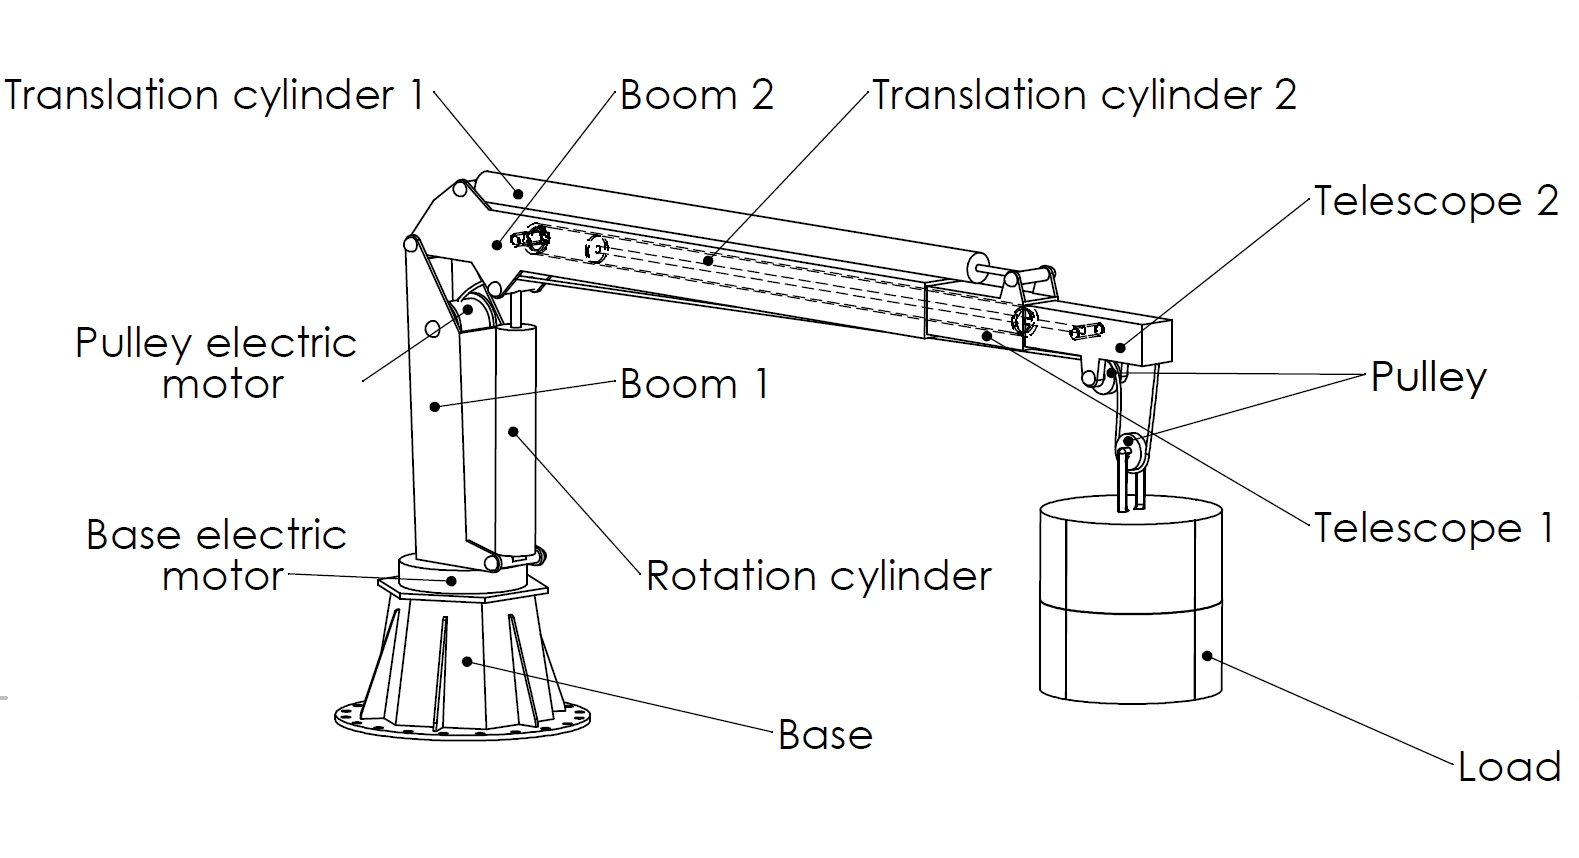
\includegraphics[width=\textwidth]{kran_teret_izometrija.jpg}
		\caption{Crane configuration, isometry.}
		\label{fig:isometry}
	\end{figure}
	
	\begin{center}
		\captionof{table}{Crane mass}\label{tab:crane_tab}
		\begin{tabular}{||c|| c || c|| c ||}
			\hline
			Part & Mass$[kg]$ & Part & Mass$[kg]$ \\
			\hline\hline
			Base + Base electric motor & 3794.43 & Rotation cylinder & 105.30\\ 
			\hline
			Boom 1 & 536.36 & Translation cylinder 1 & 199.42\\
			\hline
			Boom 2 & 807.88 & Translation cylinder 2 & 198.24\\
			\hline
			Telescope 1 & 664.18 & Pulley & 12.25\\
			\hline
			Telescope 2 & 611.33 & Pulley electric motor & 47.23\\
			\hline
		\end{tabular}
	\end{center}
	
	\subsection{Hydraulics system(5 points)}
	
	Part of the crane is actuated using hydraulic system. The system, as we 
	designed it, is shown in Figure \ref{fig:hydraulic} and we are aware it has 
	some flaws. Your first task is to think about how you could redesign the 
	system and improve its performance. Concentrate on what you can conclude 
	with what we have given you, i.e. we ask you to propose a redesign of the 
	schematics. You might want to postpone this task until you are done with 
	other tasks and have a better understanding of the system you are working 
	with.
	
	\begin{figure}[h!]
		\centering
		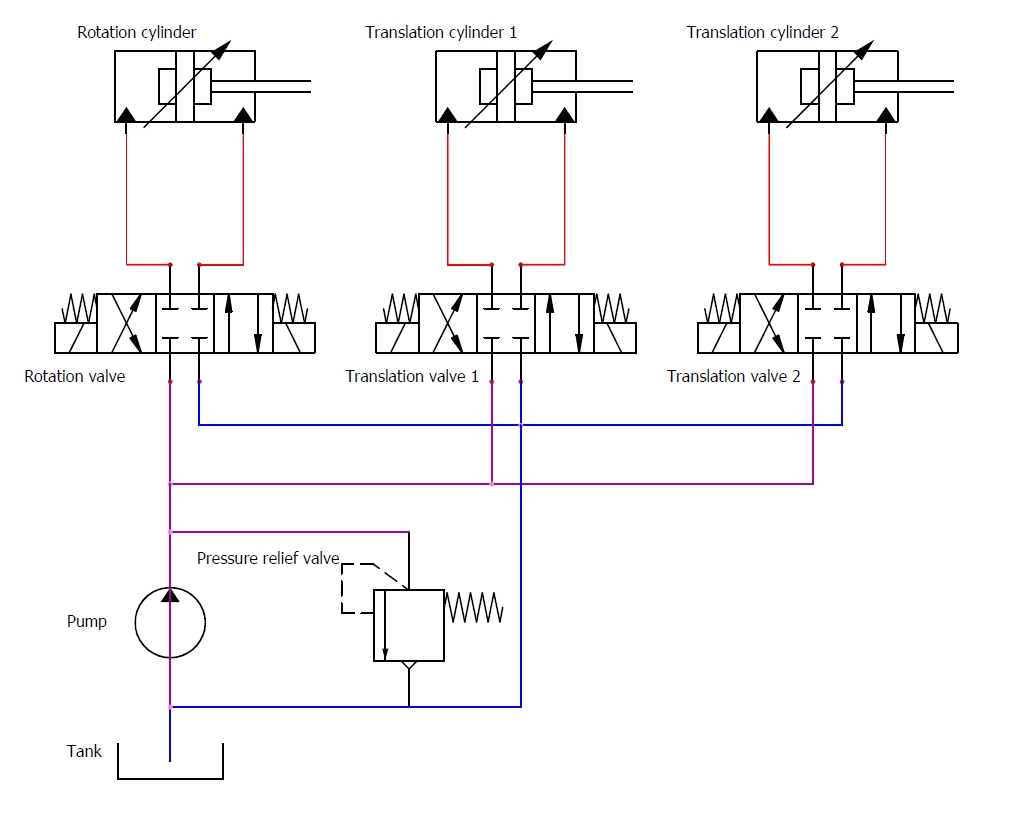
\includegraphics[width=0.75\textwidth]{hidraulika_shema.jpg}
		\caption{Hydraulic system schematics.}
		\label{fig:hydraulic}
	\end{figure}
	
	\subsection{Kinematics(20 points)}
	
	Kinematics model of the crane is important to ensure that the cargo is 
	precisely placed into the submarine which delivers it to underwater 
	habitats.
	
	Crane configuration and dimensions are shown in Figure 
	\ref{fig:crane_side}, Figure \ref{fig:crane_top} and Figure 
	\ref{fig:crane_back}. Figure \ref{fig:cylinder_conf} shows cylinder 
	configuration with corresponding dimensions given in Table 
	\ref{tab:cylinder_tab}. Load is shown in Figure \ref{fig:load}.
	
	\begin{figure}[h!]
		\centering
		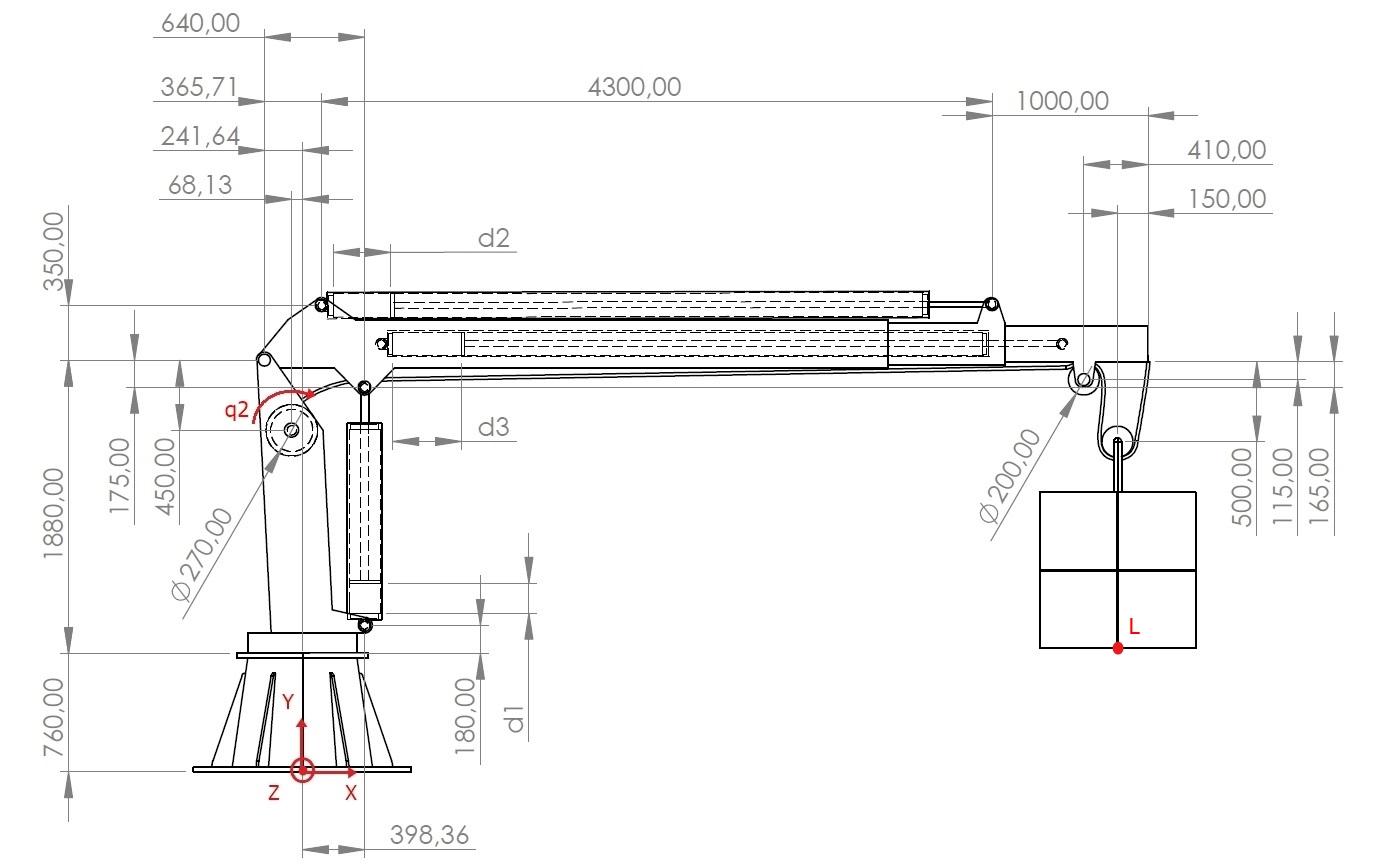
\includegraphics[width=\textwidth]{kran_bokocrt.jpg}
		\caption{Crane configuration, side view.}
		\label{fig:crane_side}
	\end{figure}
	
	\begin{figure}[h!]
		\centering
		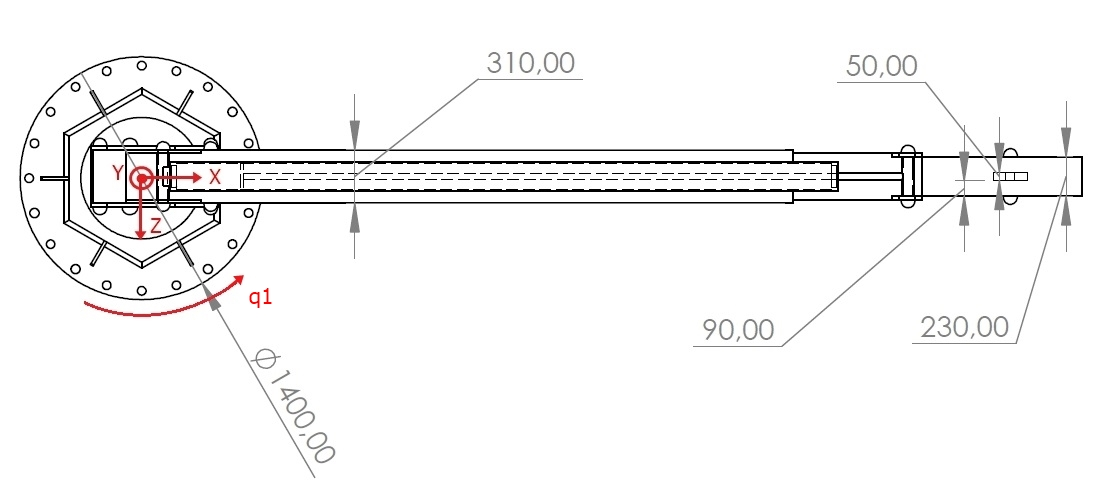
\includegraphics[width=\textwidth]{kran_tlocrt.jpg}
		\caption{Crane configuration, top view.}
		\label{fig:crane_top}
	\end{figure}
	
	\begin{figure}[h!]
		\centering
		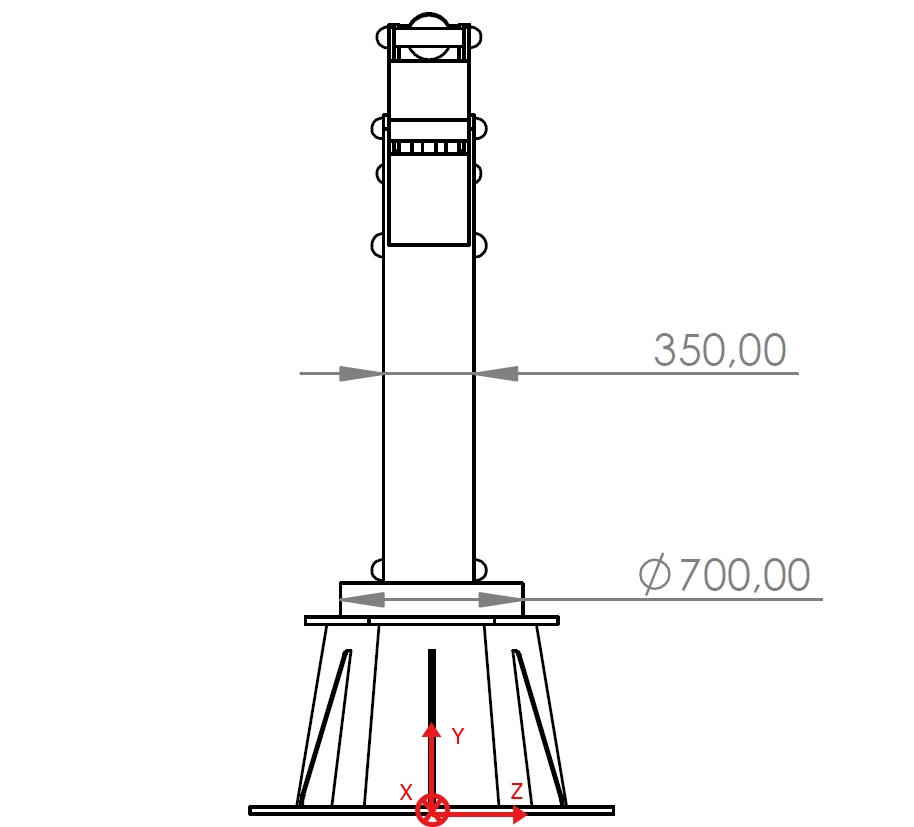
\includegraphics[width=0.65\textwidth]{kran_nacrt.jpg}
		\caption{Crane configuration, back view.}
		\label{fig:crane_back}
	\end{figure}
	
	\noindent
	\textbf{Crane configuration has been sketched for $q_1 = 0 ^\circ$, $d_1 = 
		194mm$, $d_2 = 369mm$, $d_3 = 437.22mm$ and $q_2 = 0 ^\circ$. Base 
		coordinate system is defined by red coordinate axes while red dot $L$ 
		represents bottom of the load.} Limits of motor angles and cylinder 
		offsets 
	are given in Table \ref{tab:limits}.
	
	\begin{center}
		\captionof{table}{Actuator position limits}\label{tab:limits}
		\begin{tabular}{|| c || c c c c c ||}
			\hline
			Variable & $q_1[^{\circ}]$ & $d_1$[m] & $d_2$[m] & $d_3$[m] &  
			$q_2[^{\circ}]$\\
			\hline\hline
			Minimum value & $\times$ & 0 & 0 & 0 & 0 \\ 
			\hline
			Maximum value & $\times$ & 0.8 & 3.5 & 3.5 & 20000 \\ 
			\hline
		\end{tabular}
	\end{center}
	
	\begin{figure}
		\centering
		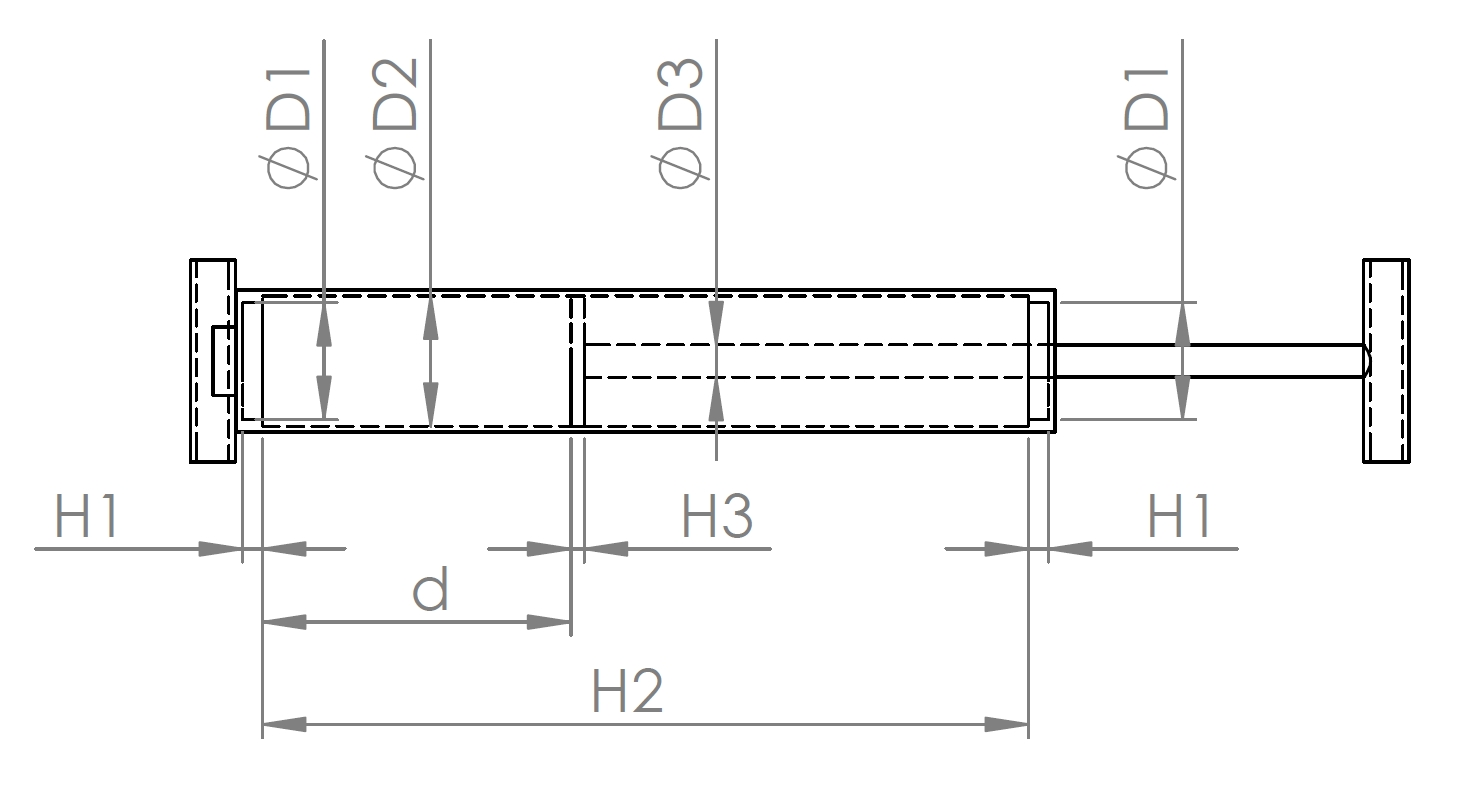
\includegraphics[width=0.75\textwidth]{cilindar_shema.jpg}
		\caption{Cylinder configuration with dimensions.}
		\label{fig:cylinder_conf}
	\end{figure}
	
	\begin{center}
		\captionof{table}{Cylinder dimensions}\label{tab:cylinder_tab}
		\begin{tabular}{||c|| c c c || c c c ||}
			\hline
			Cylinder & D1[mm] & D2[mm] &  D3[mm] & H1[mm] & H2[mm] & H3[mm] \\
			\hline\hline
			Rotation & 180 & 200 & 50 & 30 & 820 & 20\\ 
			\hline
			Translation & 80 & 100 & 37.5 & 30 & 3520 & 20 \\
			\hline
		\end{tabular}
	\end{center}
	
	\begin{figure}[h!]
		\centering
		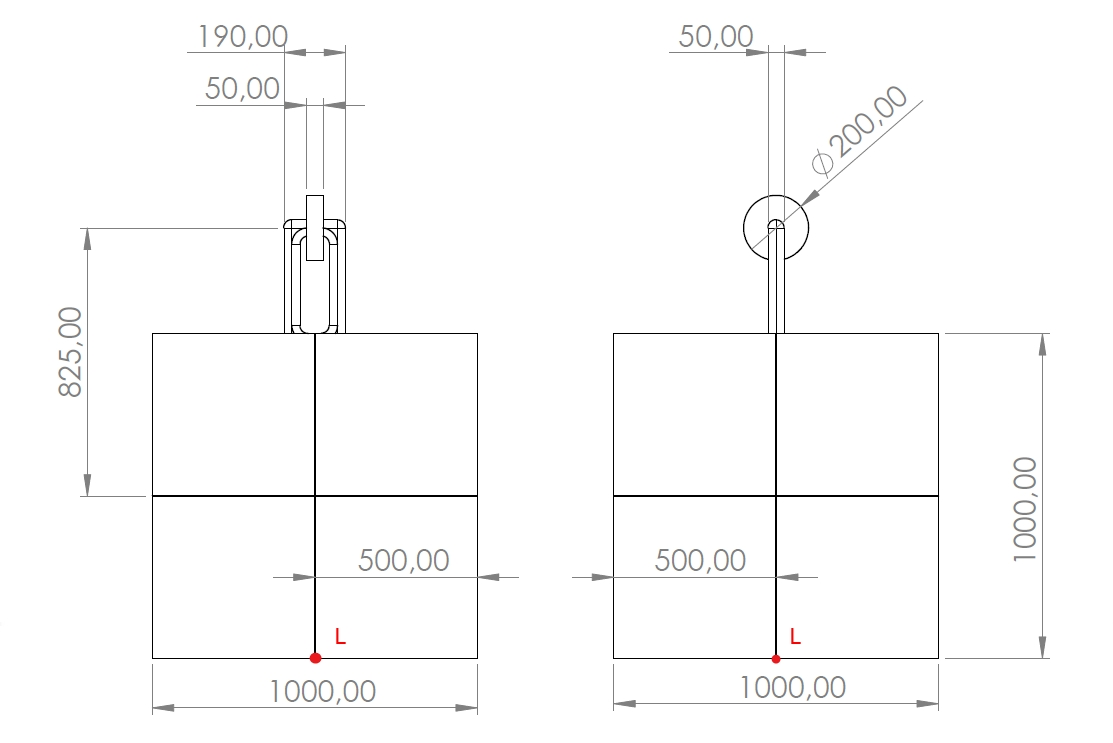
\includegraphics[width=0.8\textwidth]{teret.jpg}
		\caption{Load}
		\label{fig:load}
	\end{figure}
	
	\subsubsection{Direct}
	
	To be able to design a controller, first you have to understand  kinematics 
	of the crane. Your task is to find the position of the load 
	$L(x_L,y_L,z_L)$ for every combination of electric motor angles and 
	cylinder offsets given in Table \ref{tab:direct}. Be careful calculating 
	the result because \textbf{maximum offset} from correct solution we will 
	tolerate is $\pm 0.25$ m.
	\noindent NOTE: Pulley is trickier than it looks.
	
	
	\begin{center}
		\captionof{table}{Direct kinematics configurations}\label{tab:direct}
		\begin{tabular}{|| c || c c c c c ||}
			\hline
			Configuration & $q_1[^{\circ}]$ & $d_1$[m] & $d_2$[m] & $d_3$[m] &  
			$q_2[^{\circ}]$\\
			\hline\hline
			1. & 0 & 0.194 & 1 & 1 & 1500 \\ 
			\hline
			2. & 45 & 0.4 & 0 & 2 & 3600 \\
			\hline
			3. & 90 & 0.7 & 3.5  & 3.5 & 5000 \\
			\hline
		\end{tabular}
	\end{center}
	
	\noindent
	Information on how to submit your solution will be given to you in the 
	\textit{readme} file in task folder. If you have any questions regarding 
	submission of the task, ask your mentors.
	
	\subsubsection{Inverse}
	
	Next step is to be able to determine kinematic configuration in opposite 
	direction. Based on load positions specified in Table \ref{tab:inverse}, 
	determine the corresponding angles and offsets $(q_1, d_1, d_2, d_3, q_2)$ 
	for every given configuration. It is often the case that inverse kinematics 
	has multiple valid solutions, so any valid solution you give will be graded 
	as successful. We will set the crane in configuration position you give us 
	and check if it is inside the maximum offset range of $\pm 0.25$ m from 
	reference point given in Table \ref{tab:inverse}.
	
	\begin{center}
		\captionof{table}{Inverse kinematics configurations}
		\label{tab:inverse}
		\begin{tabular}{|| c || c c c ||}
			\hline
			Configuration & $x_L$[m] & $y_L$[m] & $z_L$[m] \\
			\hline\hline
			1. & 8.0 & -5.0 & 0.0\\ 
			\hline
			2. & -7.5 & -5.0 & 7.5 \\
			\hline
			3. & 0.0 & 0.5 & 2.5 \\
			\hline
		\end{tabular}
	\end{center}
	
	\noindent
	Information on how to submit your solution will be given to you in the 
	\textit{readme} file in task folder. If you have any questions regarding 
	submission of the task, ask your mentors.
	
	\subsection{Model identification(30 points)}
	
	Now when you understand kinematics of the crane, it would be useful to know 
	its dynamic model.
	
	As mentioned before, the crane has 5 actuators. There is a DC motor which 
	is turning the whole crane, one hydraulic actuator performing rotation of 
	booms and telescopes (lifting), two hydraulic actuators used for extension 
	of telescopes and finally a DC motor running belt and pulley system. To 
	successfully drive the crane, you have to determine how it reacts to given 
	inputs. In real systems, you often don't know how system will respond to 
	your inputs, mostly because the model of the system is unknown. In many 
	cases, there are some unknown parameters, order of model is unknown or 
	maybe some parameters are not correct due to the age of system you are 
	controlling, for example, old batteries, old motors, etc.
	
	For this task you will do exactly that! Some of the parameters of the 
	system are unknown and there is no way to measure them so you have to 
	identify models for all crane actuators.
	
	Crane is set to default start position ($q_1 = 0; \ d_1 = 0.194; \  d_2 = 
	0; \  d_3 = 0; \  q_2 = 0$) and it is ready for driving. Given the known 
	parameters of actuators (Table \ref{tab:el_params}), your job is to 
	determine how the actuator will respond. We give you the opportunity to 
	test whatever input signals you want.
	Inputs for DC motors are in Volts [V] and for hydraulic actuators are valve 
	opening in Meters[m]. Input signal limits are given in Table 
	\ref{tab:input_limits}.  In task's \textit{readme} file you can find a way 
	how to test your input signals and submit your results.
	
	\begin{center}
		\captionof{table}{Electric motor parameters}
		\label{tab:el_params}
		\begin{tabular}{|| c || c c c c c||}
			\hline
			Parameter & R[$\Omega$] & $L$[mH] & $k$[Vs/rad] & 
			$J_{rot}$[kgm$^2$] & 
			$n$\\
			\hline\hline
			Base electric motor & 2.3 & 20 & 1.3 & 0.2 & 200\\ 
			\hline
			Pulley electric motor & 1.7 & 12 & 1.6 & 0.1 & 20\\
			\hline
		\end{tabular}
	\end{center}
	
	\begin{center}
		
		\captionof{table}{Actuator input signal limits}\label{tab:input_limits}
		\begin{tabular}{|| c || c c c c c ||}
			\hline
			Actuator & \makecell{Base electric \\ motor [V]} & 
			\makecell{Rotation \\ cylinder \\ valve[m]} & \makecell{Translation 
			\\ cylinder 1 \\ valve[m]} & \makecell{Translation \\ cylinder 2 \\ 
			valve[m]} &  \makecell{Pulley electric \\ motor [V]}\\
			\hline\hline
			\makecell{Minimum \\ value} & -120 & -0.005 & -0.005 & -0.005 & 
			-180 \\ 
			\hline
			\makecell{Maximum\\ value} & 120 & 0.005 & 0.005 & 0.005 & 180 \\ 
			\hline
		\end{tabular}
	\end{center}
	
	We will test your solution with randomly generated test signals. To prevent 
	you from sending us your test signal as an input for identification, every 
	time you send signal for identification we will create new test signal and 
	\textbf{erase all your previous results}. That means that after you decide 
	that your test identification is good enough for you, you should not send 
	another identification signal.
	As said before, test signals are generated randomly. In total, you will 
	have 5 test cases.  Each test case will start in default start position . 
	Identification signal for every actuator is \textbf{step} function  
	(Heaviside function) with random step time in interval [0, $T_{sim}$] and 
	with random value amplitude. Example of one test signal can be found in the 
	task folder.
	
	\subsection{Crane driving(30 points)}
	
	After creating both kinematic and dynamic models of the system, your task 
	is to make it serve its purpose. Crane has to carry a specific cargo from 
	the dock to the submarine cargo space. Desired positions are given in Table 
	\ref{tab:inverse} and you have already calculated inverse dynamics for 
	these coordinates. Crane has to place the load in these points in the order 
	given in Table \ref{tab:trajectory}.
	
	\begin{center}
		\captionof{table}{Desired crane positions}\label{tab:trajectory}
		\begin{tabular}{|| c c c c c ||}
			\hline
			$P_1$ & $P_2$ & $P_3$ & $P_4$ & $P_5$\\
			\hline\hline
			3 & 1 & 3 & 2 & 3  \\ 
			\hline
		\end{tabular}
	\end{center}
	
	\noindent
	At each stop, the load has to stay steady for at least $t_{steady} = 5s$ 
	before proceeding to the next one. "Stay steady" in this context means that 
	the bottom point $L(x_L,y_L,z_L)$ of the load has to stay in the norm ball 
	of $R = 0.25$ m around the reference point. Test is finished after the load 
	has been in all requested positions or when the maximum simulation time 
	$T_{sim} = 250s$ has passed. This is measured using test time $T_{test}$. 
	Final performance cost $J_{total}$ is calculated using the following 
	expression:
	
	\begin{equation} \label{eq:total_cost}
	J_{total} = \frac{5}{24}\sum_{i=1}^{5} D_i + \frac{75}{2} T_{total},
	\end{equation}
	
	\begin{equation} \label{eq:distance_cost}
	D_i = \left\{
	\begin{array}{ll}
	\sum_{t=T_{i-1}}^{T_{i}} ||L(t) - P_i||, &  P_i \textrm{ reached}, \\
	& \\
	10000, &  P_i \textrm{ not reached},\\
	\end{array} 
	\right.
	\end{equation}
	
	\noindent
	where $T_i$ is the time in which $t_{steady}$ has been reached in position 
	$P_i$ and $T_0 = 0s$.
	
	\vspace{10pt}
	\noindent
	Your task is to design five controllers, one for every actuator. 
	Discretization time for every controller is $T_s = 50ms$. Information on 
	how to submit your solution will be given to you in the \textit{readme} 
	file in task folder. If you have any questions regarding submission of the 
	task, ask your mentors.
	
	\newpage
	\section{DC voltage power supply - introduction(15 points)}
	
	
	For fully functional operation, the crane is equipped with 
	lot of computer based subsystems and electronic devices which operate on DC 
	voltage. To ensure their proper operation the DC voltage has to be stable 
	and 
	without noise. To ensure stable DC voltage, device on Fig. 
	\ref{fig:schematic}. is used. Device is composed of several parts as it is 
	shown on the figure. Due to extreme conditions in the system, regulators 
	often 
	fail and components have to be repaired or replaced with proper spare part.
	
	In this task, your job is to:
	\begin{itemize}
		\item find the parts which ensure proper operation of regulator, 
		\item ensure that the output voltage ripple is within the boundaries 
		with 
		proper choice of parts for the low pass filter,
		\item find the probability of future malfunction in standby redundant 
		system.
	\end{itemize}
	
	\textbf{Device specifications.} Device specifications are provided with 
	the following table. In the first and the second task you have to choose 
	device 
	components. You have to ensure that your choice guarantees that the 
	device operating parameters are within the requirements specified in the 
	table \ref{tab:spec}.
	
	\begin{table}[h!]
		\hyphenpenalty 10000
		\caption{Device specifications}
		\label{tab:spec}
		\begin{tabularx}{\linewidth}{|X|X|X|X|} \hline
			PARAMETER & TEST CONDITIONS & VALUE & UNIT \\ \hline
			Input voltage ($U_{in}$)&  & $330$ & V \\ \hline 
			Output voltage ($U_{out}$)& $I_{out} = 1$ A & $10$ ($\pm5$) \% & V 
			\\ 
			\hline
			Output current ($I_{out}$) & $U_{in} = 330$ Vpp & $1.0$ & A \\ 
			\hline
			Ripple rejection & (36 kHz) & $78$ & dB \\ \hline
		\end{tabularx}
	\end{table}
	
	\begin{sidewaysfigure}[h!]
		\centering
		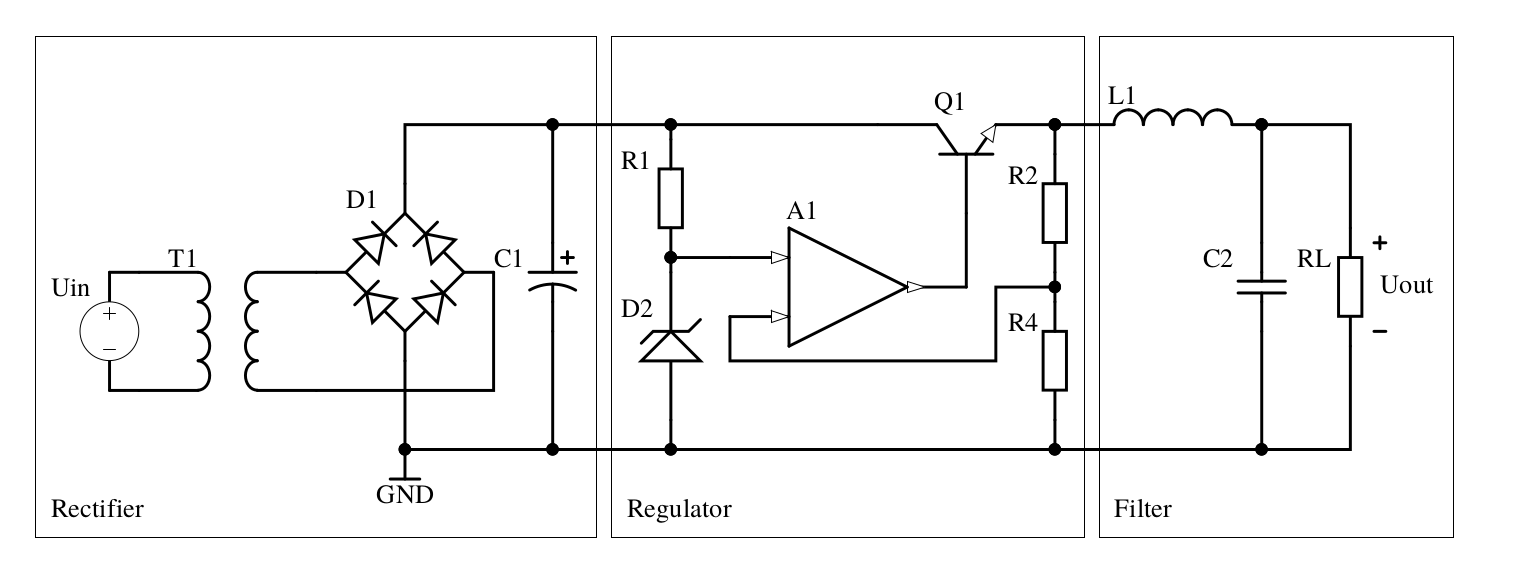
\includegraphics[width=\linewidth]{reg.png}
		\caption{DC voltage power supply device schematic}
		\label{fig:schematic}
	\end{sidewaysfigure}
	
	\clearpage
	
	\subsection{Finding the proper choice of components}
	\label{ele:task:1}
	As it can be seen from the table \ref{tab:elems}, some components are not 
	determined. 
	
	\begin{table}[h!]
		\hyphenpenalty 10000
		\caption{Device element values}
		\label{tab:elems}
		\begin{tabularx}{\linewidth}{|X|X|X|X|} \hline
			ELEMENT & PARAMETER & VALUE & UNIT \\ \hline
			$T_1$ & transfer ratio ($n$) & $25$ &  dimensionless \\ \hline
			$D_1$ & $U_{pn}$ & $0.6$ & V \\ \hline 
			$R_2$ & Resistance & $1$ & M$\Omega$ \\ \hline
			$R_4$ & Resistance & $470$ & k$\Omega$ \\ \hline
			$R_L$ & Resistance & 10 & $\Omega$ \\ \hline
			$Q_1$ & $U_{pn}$ & $0.6$ & V \\ \hline
			$C_1$ & Capacitance & $10$ & mF \\ \hline
		\end{tabularx}
	\end{table}
	In this subtask you need to specify resistor $R_1$ and diode $D_2$. Based 
	on 
	the device operating values provided with table \ref{tab:spec} you have to 
	determine specifications for the resistor $R_1$ and diode $D_2$. You have 
	to 
	find the components from the DigiKey Electronics product database. 
	
	There are, however, constraints for your choice of components:
	\begin{itemize}
		\item $R_1$ has footprint given with figure Fig. \ref{fig:footprint},
		\item $D_2$ is a through-hole component.
	\end{itemize} 
	
	Your choice is graded in several ways:
	\begin{itemize}
		\item component price,
		\item correct component voltage, power and current ratings,
		\item correct component footprint.
	\end{itemize}
	As a result, you have to provide part number for resistor and part number 
	for
	diode, respectively.
	
	\begin{figure}[h!]
		\centering
		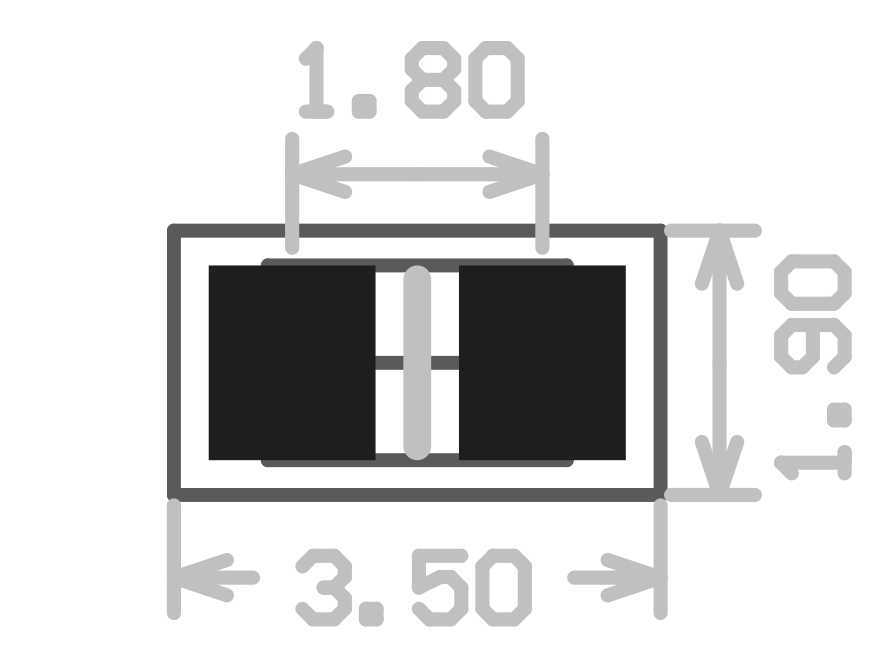
\includegraphics[width=0.5\linewidth]{footprint.png}
		\caption{Component footprint with dimension in millimeters}
		\label{fig:footprint}
	\end{figure}
	
	\newpage
	
	\subsection{LC filter design}
	\label{ele:task:2}
	To achieve specified ripple rejection at required frequency, design a LC 
	low 
	pass filter which filters output of a regulator. As in previous task you 
	have 
	to provide DigiKey part numbers for LC filter. \textbf{Note:} The ripple 
	rejection of the regulator part of the device is $58$ dB at $36$ kHz.
	
	Again, there are constraints for your choice of components:
	\begin{itemize}
		\item $L_1$ has no additional constraints 
		(think about already mentioned implicit constraints),
		\item $C_2$ has footprint given with Fig. \ref{fig:footprint},
		\item $Q$ factor has to be equal $\frac{\sqrt{2}}{2}$ for $R_L = 10$ 
		$\Omega$.  
	\end{itemize}
	$Q$ factor has to be as close to $\frac{\sqrt{2}}{2}$ as possible. 
	
	Your choice is graded in the similar fashion as before:
	\begin{itemize}
		\item price,
		\item correct inductance and capacitance,
		\item correct footprints, 
		\item correct current and voltage ratings.
	\end{itemize}
	As a result, you have to provide part number for inductor and 
	part number for capacitor, respectively. 
	\newpage
	\subsection{Side task: Reliability of the system with redundant power 
	supply} 
	\label{ele:task:3}
	To increase reliability of the power supply system two different linear 
	regulators are linked in configuration which is given with the Fig. 
	\ref{fig:psc}. This configuration is known as passive standby redundancy. 
	Probability of a failure in one regulator is modeled with exponential 
	probability density function. More precisely, probability density function 
	for 
	the first regulator is:  
	\begin{equation}
	f_1(t) = \lambda_1 e^{-\lambda_1 t}
	\end{equation}
	and for the second regulator:
	\begin{equation}
	f_2(t) = \lambda_2 e^{-\lambda_2 t}
	\end{equation}
	
	Your task is to determine probability density function $f_S(t)$ which gives 
	the
	probability of failure in system described with Fig. \ref{fig:psc}. As a 
	result 
	provide probability of a failure for $t = 10000$ $h$ with:
	\begin{itemize}
		\item[] $\lambda_1 = 1 \cdot10^{-6}$ $h^{-1}$
		\item[] $\lambda_2 = 2 \cdot10^{-6}$ $h^{-1}$ 
	\end{itemize} 
	
	\textbf{Note}: mean time between failures is increased $T_{sf} = 
	T_{1f} + T_{2f}$. 
	
	\begin{figure}[h!]
		\centering
		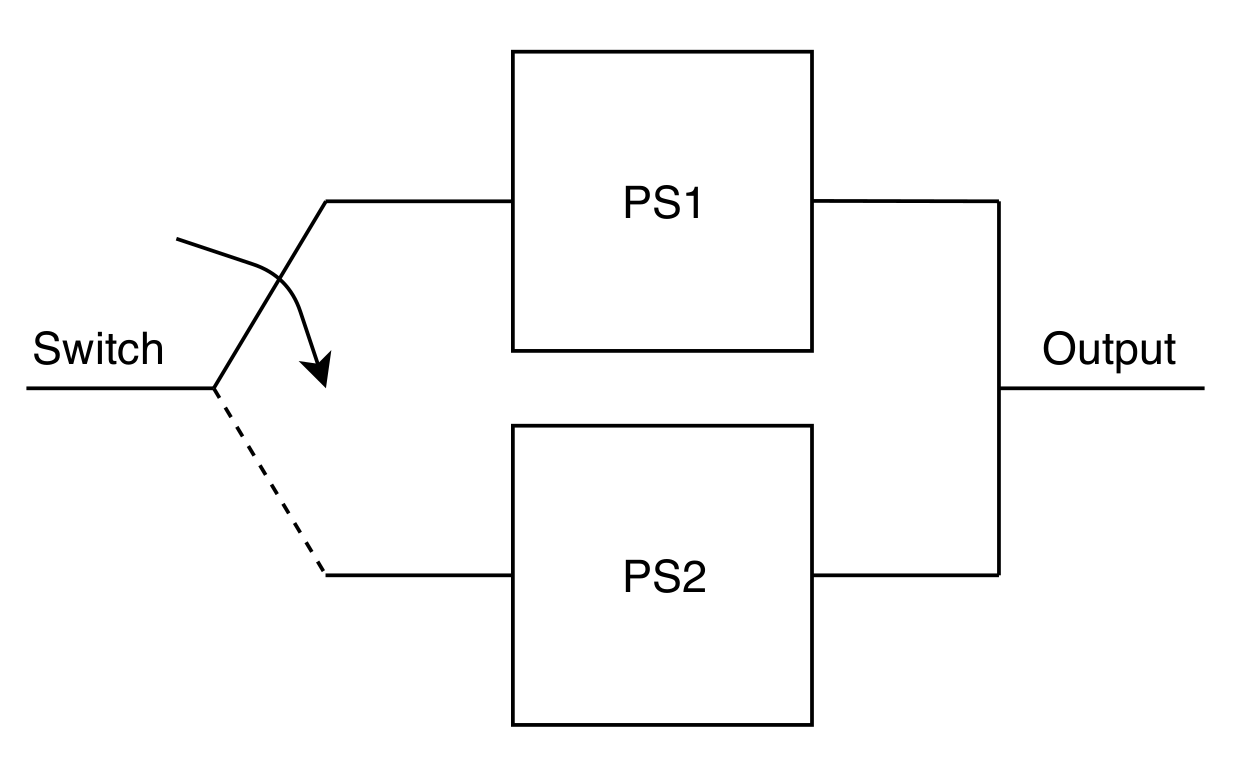
\includegraphics[width=\linewidth]{standby.png}
		\caption{Standby system configuration}
		\label{fig:psc}
	\end{figure}
	
	\newpage
	
	\subsection{Solution format}
	Solution for each task is a plain text document containing requested data. 
	For
	the tasks \ref{ele:task:1} and \ref{ele:task:2} text documents need to have 
	two rows. One component part number in each row. Only one row is needed for 
	the 
	task \ref{ele:task:3} (requested probability). Name the files 
	\texttt{task1.txt}, \texttt{task2.txt}, \texttt{task3.txt} and put them in 
	the appropriate Google Drive folder.
	
	Additionally, for the task \ref{ele:task:3} you have to provide paper 
	documentation which has to contain derivation of $f_S(t)$.
	
	\subsection{Grading scheme}
	Tasks are graded in the following manner:
	\begin{itemize}
		\item tasks \ref{ele:task:1} and \ref{ele:task:2} - up to \textbf{5 
		pts} 
		each (correct components in each task), 
		\item task \ref{ele:task:3} - up to \textbf{5 pts} - \textbf{2.5 pts} 
		for 
		the correct probability and up to \textbf{2.5 pts} for correct 
		documentation.
	\end{itemize}
	
	
	
	\chapter{Day 2}
	
	\section{Introduction}
	
	The choice of propulsion system type is one of the most important parts in 
	submarine’s design process since it determines the ability of fulfilling 
	its purpose. Submarines that perform underwater research activities require 
	endurance and certain flexibility in different littoral conditions. For 
	example, conventional motor propulsion systems, such as diesel electric, 
	when operational, require fresh air intake for driving electrical 
	generator. In this way, a period while a submarine can remain submerged is 
	limited by the power and endurance of the battery system and counts in 
	hours or few days at most. Therefore, when it comes to endurance such 
	systems might not be an optimal choice. Technology that overcomes this 
	drawback is a nuclear power system which offers better endurance (even few 
	months) and speed of the submarines but there are number of disadvantages 
	(very expensive, operational limitations in shallow littoral waters etc.) 
	that make them unsuitable for underwater research activities. The most 
	suitable seems to be so called Air Independent Propulsion systems (AIP 
	systems) which are marine propulsion technologies that allows non-nuclear 
	submarine to operate without access to atmospheric oxygen. 
	
	One of the most interesting is definitely French AIP technology so called 
	MESMA (Module d'Energie Sous-Marine Autonome). This is the AIP system that 
	uses closed-turbine cycle for powering electrical generator and the heat 
	for steam generation is provided by liquid bioethanol combustion in pure 
	oxygen. Combustion of pure bioethanol makes this system ecologically much 
	more acceptable than other systems that use conventional fuels. In this 
	way, virtually silent MESMA exploits all advantages of AIP systems for 
	maintenance of underwater habitats and performing underwater research or 
	training activities.
	
	
	The assignment can be divided into two steps: 
	
	\begin{enumerate}
		\item Design and dimension main components of the propulsion system,
		\item Define operational characteristics of some components.
	\end{enumerate}
	
	After the first step you will be given a full model of propulsion system 
	with the components you selected which will help you define operational 
	characteristics of some components.
	Detailed description of the system components is given in the next section.
	
	Engineers, good luck!
	
	\newpage
	\section{Power generation system description}
	
	
	\subsection{The submarine}
	
	Today's assignment is to design a MESMA power generation system for 
	submarine propulsion for a given submarine hull which consists of outer and 
	inner shell, showed on Figure \ref{fig:side_view}. Inside inner shell 
	there is a reserved space of fixed volume consisting of five compartments;
	power system comparment (compartment 5), bioethanol tank (compartment 4), 
	liquid oxygen tank (compartment 3), cargo storage (compartment 2), and crew 
	deck (compartment 1).
	
	
	\begin{figure}[h!]
		\centering
		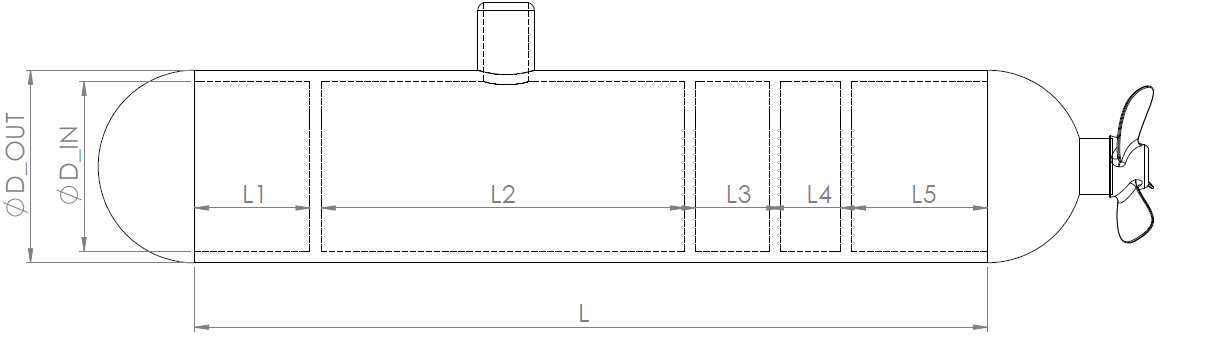
\includegraphics[width=\textwidth]{submarine_side_view.png}
		\caption{Submarine dimensions}
		\label{fig:side_view}
	\end{figure}
	
	The following dimensions are given:
	\begin{itemize}
		\item $L = 18 \,\textrm{m}$
		\item $D_{OUT} = 1.7 \,\textrm{m}$
		\item $D_{IN} = 1.5 \,\textrm{m}$
		\item $L_1 = 2 \,\textrm{m}$
	\end{itemize}
	
	$D_{IN}$  is used for the tank volume calculation.
	
	Also, dimension $L_5$ is found as
	\begin{equation}
	L_5 = (18 \cdot P_\textrm{turb} + 2500)/1000 \,\left[\textrm{m}\right]
	\end{equation}
	where the power $P_\textrm{turb}$ is taken in kW. Dimensions $L_2$ and 
	$L_3$ depend on the chosen amount of fuel and oxygen.
	
	Team's solutions will be ranked in the following categories:
	\begin{itemize}
		\item Maximum speed
		\item Maximum range
		\item Maximum depth
		\item Available cargo volume
	\end{itemize}
	Each category can win you up to 25\% of points available for this task. The 
	team that achieved the highest score in each category will be awarded the 
	maximum number of points. The other teams' points will be scaled 
	accordingly.
	
	
	
	\subsection{Power system}
	
	Power generation system schematics are shown on figure \ref{fig:pwr_scheme}.
	
	\begin{figure}[h!]
		\centering
		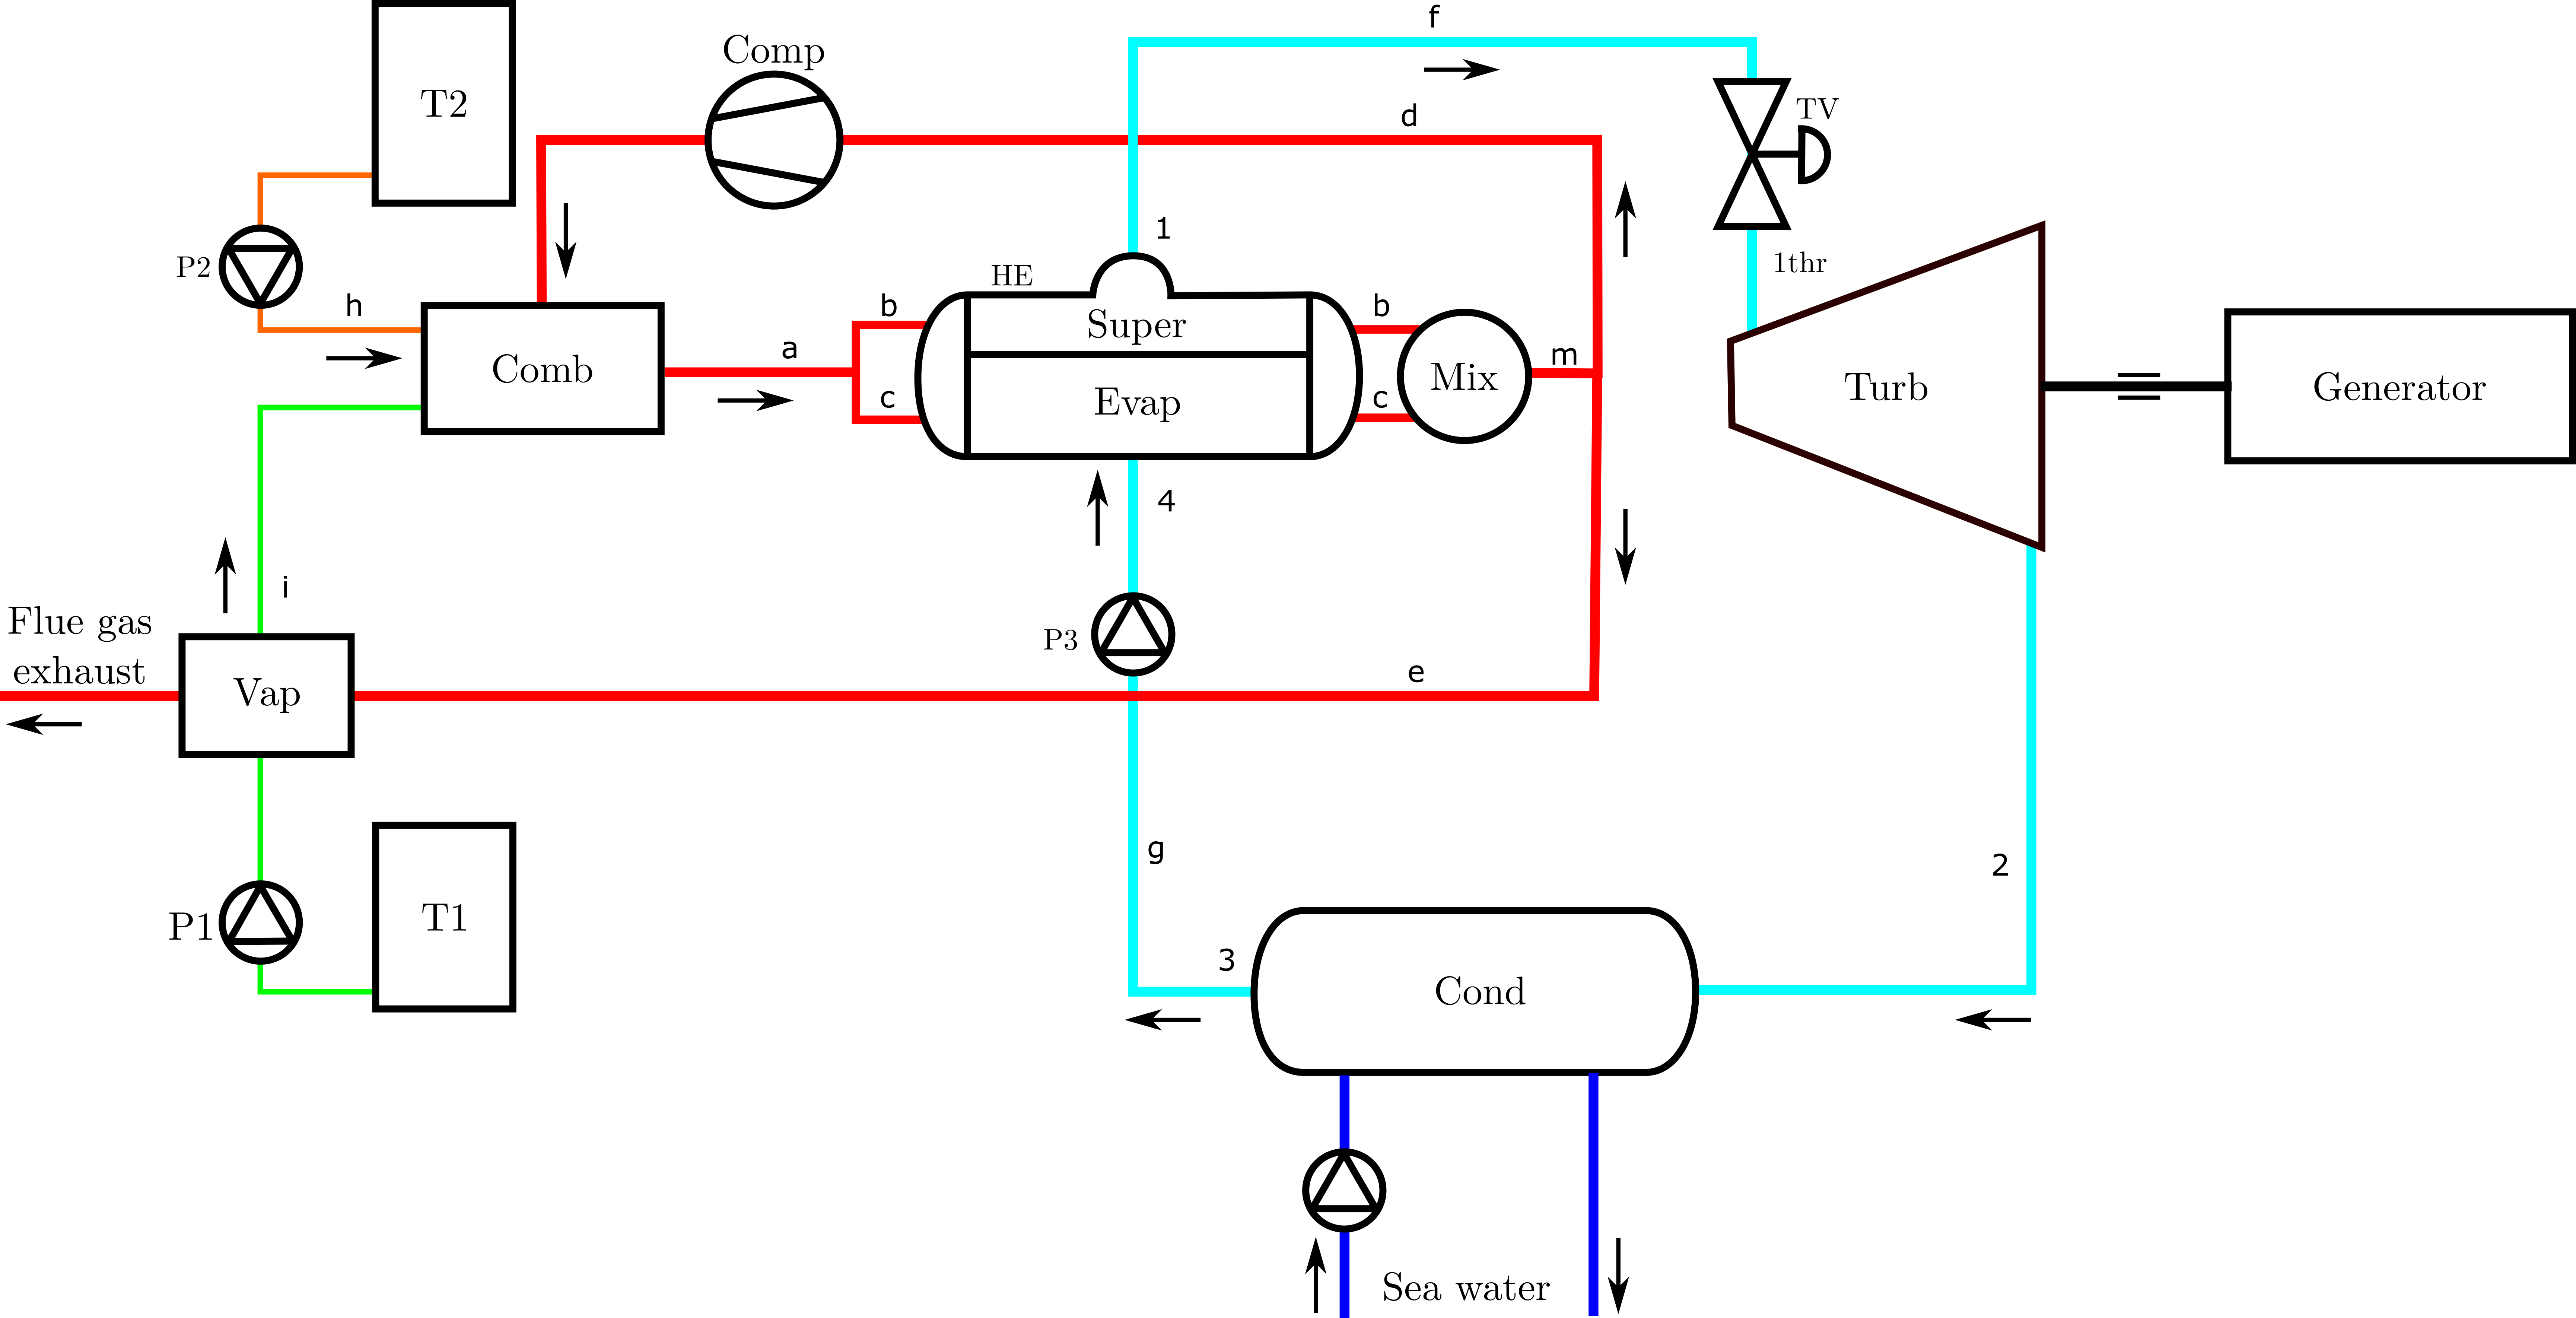
\includegraphics[width=\textwidth]{terma.png}
		\caption{Power generation system}
		\label{fig:pwr_scheme}
	\end{figure}
	
	Submarine power generation system consists of two main circuits; \\
	flue gas\footnote{combustion exhaust gas} circuit (red) and steam 
	circuit (cyan). 
	Steam circuit is used for steam production which expands in turbine "Turb" 
	providing necessary power for the "Generator" used for charging the 
	batteries for submarine propulsion. The flue gas circuit is used to provide 
	necessary heat flow for evaporating and superheating the steam for the 
	turbine. Flue gas is generated in the combustion chamber "Comb" in which 
	energy is released by ethanol combustion in pure oxygen.
	
	Liquefied oxygen and ethanol fuel are stored in separate tanks "T1" and 
	"T2", respectively. While pump P2 delivers fuel stream "h" to combustion 
	chamber "Comb", cryogenic pump P1 delivers liquefied oxygen stream "i" to 
	oxygen vaporizer "Vap" where it vaporizes and enters combustion chamber 
	"Comb" in stoichiometric ratio at which fuel combustion is, by assumption, 
	complete without any excess oxygen. Flue gas temperature at the outlet from 
	the combustion chamber (stream "a") is controlled by return stream of 
	cooled flue gas "d" by compressor "Comp" and\\
	should never exceed maximum allowed flue gas temperature %ϑ_(fg,max).
	
	Flue gas stream "a", which exits combustion chamber "Comb" enters heat 
	exchanger "HE" used for water evaporation and steam superheating. 
	Therefore, heat exchanger "HE" comprises two sections; an evaporation 
	section "Evap" and superheating section "Super". Total 
	flue gas mass flow which enters heat exchanger "HE" is divided into two 
	flue gas streams "b" and "c". Stream "c" flows through evaporation ("Evap") 
	section and stream "b" flows through superheating ("Super") section in 
	parallel configuration. On heat exchanger exit, two flue gas parallel 
	streams "b" and "c" are adiabatically mixed in mixing chamber "Mix" forming 
	flue gas stream "m".Part of stream "m" is returned by compressor "Comp" to 
	combustion chamber "Comb" as stream "d" to prevent overheating (maximum 
	allowed flue gas temperature), while the rest (stream "e") is used for 
	oxygen evaporation in heat exchanger "Vap" and evacuated outside submarine.
	
	Heat exchanger "HE" is a pool boiling type apparatus which means that 
	liquid water in the evaporating section is at rest and is evaporated by the 
	flue gas that passes through a tube bundle in the evaporating section. The 
	exact amount of steam that is evaporated in evaporation section "Evap" 
	(which corresponds to the steam mass flow of stream "g") is then 
	superheated in superheating section "Super" of heat exchanger "HE" 
	producing the superheated steam "f". Superheated steam (stream "f") passes 
	through throttling valve "TV" and enters the steam turbine "Turb" where 
	mechanical power is produced by steam adiabatic expansion to condensation 
	pressure p2. After the expansion, low pressure steam condenses in sea water 
	cooled condenser "Cond" and is returned to high pressure evaporator "Evap" 
	by condensate pump "P3". 
	
	
	Following sections provide a detailed description of every part of power 
	generation system that should be modeled.
	
	
	It is very important that system states are in allowed limits. 
	
	\begin{itemize}
		\item Maximum temperature at combustion chamber “Comb“ exit 
		(850$^\circ$)
		\item Maximum steam temperature at turbine “Turb” inlet (Excell table 1)
		\item Minimum vapor fraction on turbine “Turb” outlet (0.9)
		\item Evaporator “Evap” erosion (given by the equation 
		\ref{eq:flue_gas_density})
		\item Superheater “Super” erosion (given by the equation 
		\ref{eq:flue_gas_density})
		\item System malfunction due to insufficient generated power (given by 
		the equation \ref{eq:minpower})
	\end{itemize}
	
	Each failed test will cause 40\% point reduction in the given test category.
	
	\subsection{Turbine}
	
	A Steam Turbine is a mechanical device in which thermal energy is extracted 
	from pressurized steam by its adiabatic expansion and is transformed to 
	mechanical work.  Therefore, for a given mass flow rate of steam qm, power 
	$P$ generated by steam turbine is defined:
	
	\begin{equation}\label{eq:power}
	P = q_m(h_1 - h_2),
	\end{equation}
	
	\noindent
	where 
	
	\begin{itemize}
		\item $q_m$ is steam mass flow rate, 
		\item $h_1$ is steam specific enthalpy at turbine inlet,
		\item $h_2$ is steam specific enthalpy at turbine outlet.
	\end{itemize}
	
	Turbine steam swallowing capacity mass flow rate $q_m$ at given pressures 
	and inlet temperature can be expressed by Stodola’s Ellipse equation:
	
	\begin{equation}\label{eq:stodola}
	q_m = \frac{K}{\sqrt{T}}(p_1^2 - p_2^2)^\frac{1}{2},
	\end{equation}
	
	\noindent
	where:
	
	\begin{itemize}
		\item $K$ is Stodola’s coefficient $\left[\frac{\sqrt{\textrm{K}}\cdot 
			\textrm{kg}}{\textrm{s} \cdot \textrm{\textrm{bar}}}\right]$, 
		\item $p_1$ is turbine inlet pressure $\left[\textrm{bar}\right]$,
		\item $p_2$ is turbine outlet pressure $\left[\textrm{bar}\right]$,
		\item $T$ is turbine inlet absolute temperature 
		$\left[\textrm{K}\right]$.
	\end{itemize}
	
	\subsubsection*{Steam turbine isentropic efficiency}
	
	Turbine isentropic efficiency $\eta$ is defined as the ratio between 
	enthalpy drop at actual turbine expansion and enthalpy drop at isentropic 
	expansion between inlet and outlet turbine pressure $p_1$ and $p_2$.
	
	\begin{equation}\label{eq:eta}
	\eta = \frac{h_1-h_2}{h_1 - h_{2s}}.
	\end{equation}
	
	Steam turbine isentropic efficiency depends upon mean steam volume flow 
	rate $q_v$ according to the following equation:
	
	\begin{equation}\label{eq:eta2}
	\eta = aq_v^2 + bq_v + c,
	\end{equation}
	
	\noindent
	where $q_v$ is geometric mean of volume flow rates at turbine inlet 
	($q_{v,in}$) and at outlet in case of isentropic expansion ($q_{v,out,s}$). 
	
	\begin{equation}\label{eq:q_v}
	q_v = \sqrt{q_{v,in} \cdot q_{v,out,s}},
	\end{equation}
	
	Turbine efficiency is highest at its nominal design point for which 
	pressures ($p_1$, $p_2$) and inlet temperature T1 are given in Excel Table 
	1, while nominal flow rate is defined by Stodola’s Ellipse equation 
	\ref{eq:stodola}. Turbine can operate at other conditions (off design 
	turbine performance with lower, i.e. higher mass flow rates than the 
	nominal) with the cost of reduced efficiency, provided that these 
	conditions are not outside permitted values.
	
	\subsubsection*{Off design turbine performance}
	
	\subsubsection*{Lower mass flow rate}
	
	Steam throttling is a common way for reduction of power produced by steam 
	turbine. By reducing fuel pump "P2" and oxygen pump "P1" speed accordingly 
	when power demand is lowered, fuel consumption and evaporated steam mass 
	flow rate are decreased. In conjunction with steam flow rate decrease, 
	throttling valve "TV" orifice is constricted to reduce turbine inlet 
	pressure $p_{1,thr}$ to a value which satisfies Stodola’s Ellipse law 
	\ref{eq:stodola} for given decreased mass flow rate $q_m$. In a throttling 
	process, superheated steam which exits heat exchanger "HE" is throttled to 
	lower pressure $p_{1,thr}$, while steam enthalpy is conserved.
	
	\begin{equation}\label{eq:ent_preserve1}
	h_{1,thr} = h_1,
	\end{equation}
	\begin{equation}\label{eq:ent_preserve2}
	p_{1,thr} = p_1,
	\end{equation}
	\begin{equation}\label{eq:ent_preserve3}
	T_{1,thr} = T(p_{1,thr},h_1) < T_1.
	\end{equation}
	
	Side effect of throttling is a temperature reduction which corresponds to 
	the state of conserved enthalpy $h_1$ at throttled pressure $p_{1,thr}$. 
	Pressure and temperature are both part of a Stodola’s Ellipse law 
	\ref{eq:stodola} which means they need to simultaneously satisfy Stodola’s 
	Ellipse law  \ref{eq:stodola}  and enthalpy conservation of a throttling 
	process from state "1".
	
	By throttling, turbine inlet pressure and inlet temperature are reduced 
	which decreases available isentropic power of turbine. Turbine efficiency 
	described by equation \ref{eq:eta2} is also decreased at partial turbine 
	load.
	
	\subsubsection*{Higher mass flow rate}
	
	In case that power demand is increased, turbine can be overloaded by steam 
	mass flow $q_m$ greater than nominal. This is achieved by fuel pump "P2" 
	and oxygen pump "P1" speed increase which causes increased fuel consumption 
	and evaporated steam mass flow. When turbine is overloaded, steam flow 
	bypasses few initial turbine stages which enables increased steam 
	consumption, although with reduced turbine efficiency described by equation 
	(4). To accurately model this effect is out of scope of this assignment. 
	Therefore, it is assumed in overload working mode that turbine inlet values 
	of pressure and temperature remain nominal, i.e. there is no change at 
	throttling valve due to increased steam mass flow rate $q_m$. The only 
	effect of increased $q_m$ is turbine efficiency reduction as described by 
	equation \ref{eq:eta2}.
	
	Restrictions of steam turbine operational parameters are following:
	
	\begin{itemize}
		\item Steam temperature at turbine inlet should not exceed temperature 
		$\vartheta_{turb,max}$,
		\item Define operational characteristics of some components.
	\end{itemize}
	
	\noindent
	\textcolor{red}{Turbine design parameters are given in Excel Table 1.}
	
	\subsubsection*{Minimum required turbine power}
	
	The minimum power which the turbine has to provide for the submarine for it 
	to remain operational is defined by
	\begin{equation}\label{eq:minpower}
	P_\textrm{min} = 2 + 0.05 \cdot P_\textrm{nom} \ \left[\textrm{kW}\right]
	\end{equation}
	where $P_\textrm{nom}$ is the nominal turbine power, given in Excel Table 1 
	in kW.
	
	If the power generated by the turbine falls below the value of 
	$P_\textrm{min}$, the submarine will fatally malfunction.
	
	Submarine velocity is calculated based on the power remaining for 
	propulsions, as
	\begin{equation}
	v_\textrm{sub} = 2.0135 \cdot P_\textrm{prop}^{0.3518} \ 
	\left[\textrm{kn}\right]
	\end{equation}
	where $P_\textrm{prop}$ is taken in kW, and it is equal to
	\begin{equation}
	P_\textrm{prop} = P_\textrm{turb} - P_\textrm{min}
	\end{equation}
	
	\subsection{Heat exchangers}
	
	Heat exchanger is a device whose purpose is to transfer heat from warmer 
	fluid stream to colder stream. There are three heat exchangers in the power 
	generation system: heat exchanger "HE" which is divided to superheating and 
	evaporative section, condenser "Cond" and oxygen vaporizer "Vap". Condenser 
	"Cond" and vaporizer "Vap", whose performance will not be evaluated in this 
	task are assumed to be regulated accordingly in each time step with the 
	current need of the power generation system. 
	
	\subsubsection*{Heat exchanger "HE"}
	
	Heat exchanger "HE" is used for steam evaporation and superheating in two 
	corresponding sections by hot flue gas from combustion chamber ("b" and "c" 
	stream). It is shell and tube type with flue gas passing through tubes in 
	each section. 
	
	Heat flow exchanged in each of two heat exchanger sections is described as:
	
	\begin{equation}\label{eq:heat_flow}
	\Phi = A \cdot k \cdot LMTD,
	\end{equation}
	
	where:
	
	\noindent
	$LMTD$ is logarithmic mean temperature difference, 
	$k$ is overall heat transfer coefficient,
	$A$ is total heat exchange area of the section. 
	Assume superheating section of heat exchanger is counter-flow.
	
	In addition to LMTD method, rate of heat transfer can be determined using 
	NTU method. For counter-flow heat exchanger effectiveness is calculated as:
	
	\begin{equation}\label{eq:heat_exchanger_eff}
	\pi_1 = \frac{1 - exp((1-\pi_3)\pi_2)}{1-\pi_3exp(-(1-\pi_3)\pi_2)},
	\end{equation}
	
	Dimensionless parameters $\pi_1$,$\pi_2$,$\pi_3$ are defined as follows:
	
	\begin{equation}\label{eq:pi_params}
	\pi_1 = \frac{\theta'_1 - \theta''_1}{\theta'_1 - \theta'_2},
	\end{equation}
	
	\begin{equation}\label{eq:pi_params2}
	\pi_2 = \frac{kA}{C_1},
	\end{equation}
	
	\begin{equation}\label{eq:pi_params3}
	\pi_3 = \frac{C_1}{C_2},
	\end{equation}
	
	\noindent
	where $C$ is stream heat capacity.
	
	Index 1 corresponds to stream with lower heat capacity, index 2 to stream 
	with higher heat capacity, superscript $'$ to stream inlet state in heat 
	exchanger and $''$ to outlet state.
	
	Flue gas, which is divided into two streams "b" and "c" enters evaporation 
	"Evap" and superheating "Super" section at equal temperature and flows 
	through tubes in one pass. Flue gas mass flow through evaporative and 
	superheating section of heat exchanger is defined as:
	
	\begin{equation}\label{eq:flue_gas_flow1}
	q_{m,fg,evap} = evap_{fr} \cdot q_{m,fg},
	\end{equation}
	
	\begin{equation}\label{eq:flue_gas_flow2}
	q_{m,fg,super} = (1-evap_{fr}) \cdot q_{m,fg},
	\end{equation}
	
	\noindent
	Where:
	$evap_{fr}$ is flue gas fraction of stream "c" to total flue gas stream 
	"a"  total flue gas mas flow and is assumed constant throughout system 
	operation. Its value can be selected between 0 and 1.
	$q_{m,fg}$ is total flue gas mass flow rate (stream "a") .
	$q_{m,fg,evap}$ is evaporation section mass flow rate (stream "b")
	$q_{m,fg,super}$ is superheating section mass flow rate (stream "c")
	Heat transfer coefficient on tube side can be calculated by using following 
	simplified convection models.
	
	\noindent
	If the flow is transient or turbulent ($2300 < Re < 5e6$) , mean Nusselt 
	number is defined as:
	
	\begin{equation}\label{eq:nusselt}
	Nu = \frac{f/8 \cdot (Re - 1000) \cdot Pr}{1+12.7\sqrt{f/8} \cdot 
	(Pr^{2/3}-1)},
	\end{equation}
	
	\noindent
	where $f$ is the friction factor, defined as
	
	\begin{equation}\label{eq:fric_factor}
	f = \frac{1}{(1.82\log_{10}Re - 1.64)^2}.
	\end{equation}
	
	\noindent
	If the flow is laminar ($Re<2300$), mean Nusselt number is defined as:
	
	\begin{equation}\label{eq:nusselt2}
	Nu = 1.86 \left(Pe \frac{d}{L}\right)^{1/3}.
	\end{equation}
	
	\noindent
	In above equations non-dimensional numbers are
	
	\begin{itemize}
		\item $Nu = \frac{\alpha d}{\lambda}$ Nusselt number
		\item $Re = \frac{\rho w d}{\mu}$ Reynolds number
		\item $Pr = \frac{\mu c_p}{\lambda}$ Prandtl number
		\item $Pe = Re Pr$ Peclet number
	\end{itemize}
	
	\noindent
	Nusselt, Prandtl and Reynolds numbers and flue gas velocity are calculated 
	using mean flue gas temperature properties between pipe inlet and outlet. 
	All physical properties except density are assumed independent of pressure 
	and its values for pure gases are given in appendix. Flue gas physical 
	properties are calculated as molar average of gases which form flue gas. 
	Density is calculated using ideal gas equation of state.
	
	\noindent
	Evaporation occurs on shell side of evaporative section of heat exchanger. 
	Evaporative heat transfer coefficient on shell side is assumed constant and 
	its value is $\alpha_{ev}=3500 \frac{W}{m^2 K}$. In superheater section of 
	exchanger, heat transfer coefficient on shell side is also assumed constant 
	and its value is $\alpha_{super}=70 \frac{W}{m^2 K}$.
	
	Evaporated steam mass flow $q_m$ is determined by heat flow $\Phi_e$ 
	exchanged in evaporative part "Evap" of heat exchanger "HE":
	
	\begin{equation}\label{eq:evap_steam_mass}
	\Phi_e = q_m(h'' -h_4),
	\end{equation}
	
	where $h''$ is saturated (dry) steam specific enthalpy, and $h_4$ is 
	enthalpy of subcooled liquid at condensate pump outlet. 
	The same amount of heat flow is received from stream "b" flue gas whose 
	enthalpy decreases.
	
	\begin{equation}\label{eq:evap_steam_mass2}
	\Phi_e = q_{m,fg,evap} (h_{fg,comb} - h_{fg,evap,out}),
	\end{equation}
	
	\noindent
	where 
	$h_{fg,comb}$ is flue gas specific enthalpy at combustion chamber "Comb" 
	outlet
	$h_{fg,evap,out}$ is flue gas specific enthalpy at evaporative section 
	"Evap" outlet.
	Flue gas mean molar heat capacities are given in appendix
	It is assumed that mass flow $q_m$ in current time step flows through 
	superheating section "Super" of "HE", turbine "Turb", condenser "Cond" and 
	condensate pump "P3".
	
	Evaporated steam mass flow $q_m$, whose value is determined by equation 
	(13) is then superheated at constant pressure in superheater section 
	"Super" of heat exchanger "HE" by exchanged heat flow:
	
	\begin{equation}\label{eq:evap_steam_mass3}
	\Phi_s = q_m(h_1 - h''),
	\end{equation}
	
	The same amount of heat flow is received from stream "c" flue gas whose 
	enthalpy decreases.
	
	\begin{equation}\label{eq:evap_steam_mass4}
	\Phi_s = q_{m,fg,super} (h_{fg,comb} - h_{fg,super,out}),
	\end{equation}
	
	\noindent
	where $h_{super,out}$ is flue gas specific enthalpy at superheating section 
	"Super" exit. Both flue gas streams are adiabatically mixed at heat 
	exchanger outlet in mixing chamber "Mix". Outlet temperature from the 
	mixing chamber is defined by equation:
	
	\begin{equation}\label{eq:outlet_temp}
	\Theta_{fg,ret} = \frac{q_{m,fg,evap} \cdot h_{fg,evap,out} + 
	q_{m,fg,super} \cdot h_{fg,super,out}}{q_{m,fg} \cdot c_{p,fg} 
	(\Theta_{fg,ret})},
	\end{equation}
	
	\noindent
	where:
	
	\begin{itemize}
		\item $q_{m,fg}$ is temperature after stream "b" and "c" mixing at 
		which part of flue gas is returned to combustion chamber
		\item $c_{p,fg} (\Theta_{fg,ret})$ is mean specific heat capacity of 
		flue gas between temperature $\Theta_{fg,ret}$ and $0^{\circ}C$.
	\end{itemize}
	
	Pipe diameter and thickness are given in section \ref{sec:const}.
	
	\noindent
	Value of exchanged heat at both sections depends upon stream inlet 
	conditions, overall heat transfer coefficient k and overall heat transfer 
	area A. Heat transfer coefficient k and area A are influenced by number of 
	tubes in each section and its length which define tube side heat exchanger 
	coefficient and total heat transfer area.
	
	Type and length of tubes at evaporative and superheating section are equal. 
	Number of tubes for each section and flue gas fraction which enters each 
	section can be selected independently.  
	
	While designing a heat exchanger, to prevent tube erosion, one must 
	consider that product of flue gas density, $\rho$, and squared velocity, 
	$w^2$, never exceed $6800$  Pa,  i.e. 
	
	\begin{equation}\label{eq:flue_gas_density}
	\rho w^2 < 6800 Pa.
	\end{equation}
	
	\subsubsection*{Condenser}
	
	\noindent
	Condenser "Cond" is a heat exchanger which is used for condensation of 
	steam which exits turbine "Turb" at condensation pressure $p_2$. During 
	condensation, following heat flow is released:
	
	\begin{equation}\label{eq:heat_flow_cond}
	\Phi_{cond} = q_m (h_2 - h'),
	\end{equation}
	
	\noindent
	where $h'$ is enthalpy of saturated liquid water at condensation pressure 
	$p_2$.
	
	\noindent
	Heat flow $\Phi_{cond}$ is rejected to sea water inside condenser "Cond". 
	It can be assumed that condenser "Cond" in the system is properly designed 
	and sea water mass flow at pump "P4" is automatically adjusted to absorb 
	heat flow $\Phi_{cond}$. Therefore, sizing of condenser "Cond" and sea 
	water pump "P4" and its control is not a part of this task and is assumed 
	as ideal. Condensed water always exits condenser "Cond" at saturated liquid 
	state.
	Maximum sea water temperature at which submarine has to operate is 
	$30^{\circ}C$, and minimal temperature difference between condensing steam 
	and sea water for given condenser is $15^{\circ}C$. 
	
	\subsection{Combustion chamber}
	
	Combustion chamber "Comb" is enclosed space in which ethanol burns in 
	liquid oxygen. It is assumed to be perfectly insulated. During the 
	combustion, lower heating value of ethanol is converted into flue gas 
	enthalpy. Combustion pressure is at least 1 bar above static pressure 
	evaluated at submarine centerline. Pressure loss from combustion chamber 
	"Comb" to heat exchanger "HE" can be neglected.
	
	In addition to ethanol combustion, combustion chamber "Comb" is used for 
	mixing newly formed flue gas and cooled flow gas which passed heat 
	exchanger "HE" and is returned to chamber "Comb" to prevent overheating. 
	Combustion chamber inlet streams are pure oxygen stream "i" and ethanol 
	stream "h", both at $10^{\circ}C$ and returning flue gas stream "d" at heat 
	exchanger exit temperature  $\Theta_{fg,ret}$. The only outlet stream from 
	the combustion chamber "Comb" is flue gas stream "a" which consists of 
	return flue gas "d" and flue gas newly formed by combustion. 
	
	\begin{equation}\label{eq:flue_gas_stream_new}
	q_{m,fg} = q_{m,fg,new} + q_{m,fg,ret},
	\end{equation}
	
	\noindent
	Flue gas outlet temperature is defined by first law of thermodynamics 
	applied to combustion chamber "Comb":
	
	\begin{equation}\label{eq:flue_gas_out_temp}
	\Theta_{fg,comb} = \frac{\dot{H}_{O2,in} + \dot{H}_{ethanol,in} 
	+\dot{H}_{fg,ret} + q_{n,ethanol} \Delta H_{md}}{C_{fg}},
	\end{equation}
	
	\noindent
	where
	
	\begin{itemize}
		\item $\Delta H_{md}$ is ethanol lower heating value [kJ/kmol]
		\item $\dot{H}_{O2,in}$ is enthalpy of oxygen stream "i" at $10^\circ C$
		\item $\dot{H}_{ethanol,in}$ is enthalpy of ethanol stream "h" at 
		$10^\circ C$
		\item $\dot{H}_{fg,ret}$ is enthalpy of returning flue gas at 
		temperature $\Theta_{fg,ret}$
		\item $q_{n,ethanol}$ is molar flow rate of ethanol stream "h"
		\item $C_{fg}$ is mean isobaric heat capacity of flue gas stream "a" 
		which exits combustion chamber "Comb"
	\end{itemize}
	
	\noindent
	Flue gas composition is the same in all system parts and is defined by 
	complete combustion of ethanol in pure oxygen.
	
	\subsection{Fuel and oxygen pumps}
	
	Fuel pump "P2" is used to transport fuel to combustion chamber. Pump "P2" 
	has a variable frequency drive which allows precise control of fuel mass 
	flow to combustion chamber. It is assumed that combustion of delivered fuel 
	mass flow is complete and instantaneous. It is also assumed that control of 
	oxygen pump "P1" is linked to pump "P2" in a way that oxygen supply is in 
	exact stoichiometric ratio needed for complete ethanol combustion. 
	Therefore, oxygen pump "P1" dimensioning and control is not a part of this 
	assignment. 
	Fuel pump "P2" speed determines the fuel combustion rate and influences 
	evaporation and superheating of steam in heat exchanger "HE" and finally 
	power P extracted at steam turbine "Turb".
	
	\subsubsection*{Fuel pump}
	
	Fuel pump "P2" is positive displacement pump with variable speed drive. It 
	is used to transport fuel from fuel tank "T2" to combustion chamber "Comb". 
	The total differential head a pump must generate is a sum of static head 
	difference and frictional head losses: 
	
	\begin{equation}\label{eq:head_total}
	h_{tot} = h_{stat} + h_{fr}.
	\end{equation}
	
	There is no height difference between fuel tank "T2" and combustion chamber 
	"Comb". Fuel is stored at pressure of 1 atm.
	Frictional head loss is calculated based on fuel volume flow rate:
	
	\begin{equation}\label{eq:head_loss}
	h_{fr} = k_{pipe} \cdot q_{v,fuel}^2,
	\end{equation}
	
	\noindent
	where
	
	\begin{itemize}
		\item $k_{pipe}$ is pipe friction coefficient $\left[ \frac{mh^2}{l^2} 
		\right]$
		\item $q_{v,fuel}^2$ is fuel volume flow rate
	\end{itemize}
	
	\noindent
	It is assumed that positive displacement pump volume flow rate depends only 
	on pump speed and does not depend on pump head. Pump slippage is neglected. 
	Pump volume flow rate with respect to pump speed is defined:
	
	\begin{equation}\label{eq:pump_vol_flow}
	q_v = \frac{N}{N_{max}} q_{v,max},
	\end{equation}
	
	\noindent
	where
	
	\begin{itemize}
		\item $N$ is pump speed
		\item $N_{max}$ is maximum pump speed
		\item $q_{v,max}$ is maximum pump volume flow rate.
	\end{itemize}
	
	\noindent
	Pump head is limited to $h_{max}$. Pump speed is limited at given submarine 
	depth such that pump total head does not exceed maximum head:
	
	\begin{equation}\label{eq:total_head_limit}
	h_{stat} + k_{pipe} \left( \frac{N}{N_{max}} q_{v,max} \right)^2 \leq 
	h_{max}.
	\end{equation}
	
	\noindent
	\textcolor{red}{Pump parameters are given in Excel Table 3.}
	
	\subsection{Compressor}
	
	Part of flue gas at heat exchanger exit after mixing at mixing chamber 
	"Mix" is returned to combustion chamber "Comb" by compressor "Comp". This 
	flue gas return should ensure that flue gas stream "a" always exits 
	combustion chamber at temperature below $\theta_{fg,max}$. Compressor 
	"Comp" can provide any flue gas mass flow rate between minimum and maximum 
	flow rate defined for that compressor type. It can be assumed that 
	sufficient mass of flue gases is always available for return at mixing 
	region "Mix".
	
	Compressor is controlled with respect to fuel pump speed.  Dependence 
	between pump speed and return flue gas flow rate provided by the compressor 
	is linear. 
	
	For fully defining correlation between compressor and pump, compressor 
	loads $L_{Comp}$ at two relative pump speed $N_{rel,1}$ and $N_{rel,2}$ 
	have to be provided. Compressor load can have a value between zero and one 
	and is defined as:
	
	\begin{equation}\label{eq:compressor_load}
	L_{Comp} = \frac{q_{m,ret} - q_{m,ret,min}}{q_{m,ret,max} - q_{m,ret,min}},
	\end{equation}
	
	\noindent
	where
	
	\begin{itemize}
		\item $q_{m,ret}$ is flue gas mass flow rate which compressor "Comp" 
		returns to combustion chamber "Comb"
		\item $q_{m,ret,min}$ is minimal compressor mass flow rate
		\item $q_{m,ret,max}$ is maximal compressor mass flow rate	
	\end{itemize}
	
	\noindent
	Compressor load at some relative pump speed $N_{rel}$ is than:
	
	\begin{equation}\label{eq:compressor_load_rel}
	L_{Comp} = L_{Comp,1} + \frac{L_{Comp,2} - L_{Comp,1}}{N_{rel,2} - 
	N_{rel,1}} \left( N_{rel} - N_{rel,1}\right)
	\end{equation}
	
	\noindent
	and is bounded between values 0 and 1.
	
	\noindent
	\textcolor{red}{Compressor parameters are given in Excel Table 2.}
	
	\subsection{Condensate pump}
	
	Condensate pump "P3" is used for return of condensed steam at low 
	condensation pressure $p_3$ condenser "Cond" outlet to heat exchanger "HE" 
	at high evaporation pressure $p_4$.
	Specific enthalpy $h_4 = 359.83 \,\textrm{kJ/kg}$ at pump outlet.
	
	\subsection{Constants} \label{sec:const}
	
	\begin{itemize}
		\item $\theta_\textrm{fg,max} = 850 ^\circ C$
		\item $d_\textrm{pipe} = 20 \,\textrm{mm}$
		\item $\delta_\textrm{pipe} = 2 \,\textrm{mm}$
		\item $\lambda_\textrm{pipe}  = 58 \,\textrm{W/mK}$
		\item $Re_\textrm{crit} = 2300$
		\item $\alpha_\textrm{ev} = 3500 \frac{W}{m^2K}$
		\item $\alpha_\textrm{super} = 70 \frac{W}{m^2K}$
		\item $\theta_\textrm{fuel,in} = 10 ^\circ C$
		\item $\theta_{O_2,in} = 10 ^\circ C$
		\item $M_\textrm{ethanol} = 46 \frac{kg}{kmol}$
		\item $M_{CO_2} = 44 \frac{kg}{kmol}$
		\item $M_{H_2O} = 18 \frac{kg}{kmol}$
		\item $\Delta h_\textrm{md} = 1366940 \frac{kJ}{kmol}$
		\item $C_{mp,C_2H_6O} = 2.503 \,\frac{kJ}{kmol \cdot K}$
		\item $\rho_\textrm{sea\ water} = 1000 \frac{kg}{m^3}$
		\item $\rho_\textrm{ethanol} = 789 \frac{kg}{m^3}$
		\item $\rho_\textrm{oxygen,l} = 1141 \frac{kg}{m^3}$
	\end{itemize}
	
	\noindent
	\textcolor{red}{Fluid gas properties are given in Excel Table 4.}
	
	\clearpage
	
	\section{Beamforming system introduction}
	
	An underwater habitat connects wirelessly to a ship on the surface by means 
	of 
	ultrasonic hydrophones installed at the top of the habitat. In order to 
	increase communications range, multiple hydrophones can be used to make a 
	beamforming system. A flat rectangular area, 45 cm x 45 cm in dimension, is 
	provisioned for this purpose. The area lies in the y-z plane of the 
	reference 
	coordinate system, as depicted in Figure \ref{fig:coord}.
	\begin{figure}[h!]
		\centering
		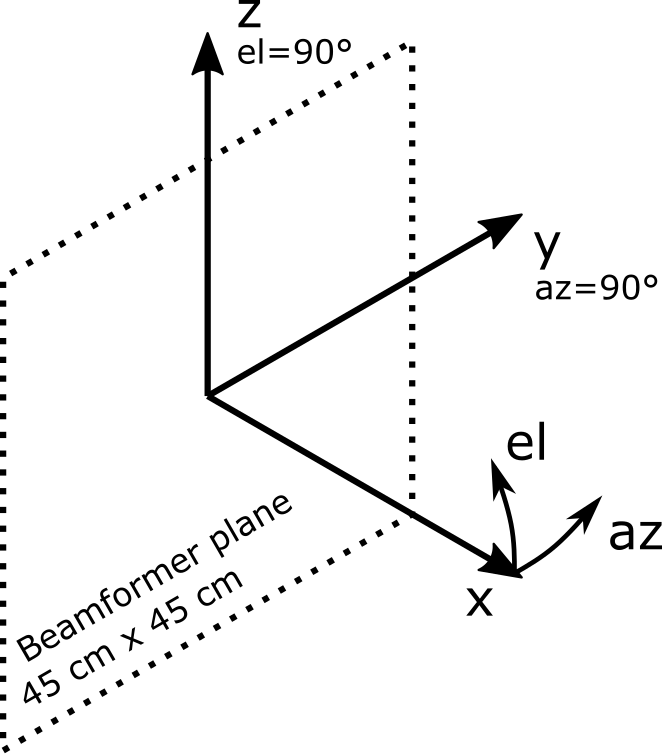
\includegraphics[width=0.4\textwidth]{coord.png}
		\caption{Reference coordinate system with available beamformer area}
		\label{fig:coord}
	\end{figure}
	
	Hydrophone operates in frequency range of 20 kHz to 90 kHz. The 
	communication 
	link uses a carrier frequency of 30 kHz. Hydrophone has a cosine radiation 
	pattern, described by expression
	\[ D(\phi,\theta) = \cos^2(\theta) \]
	with $\phi$ being azimuth angle, and $\theta$ elevation angle. The 
	radiation 
	pattern is presented in the reference coordinate system in Figure 
	\ref{fig:hydrophone}.
	\begin{figure}[h!]
		\centering
		\subfigure[3D 
		view]{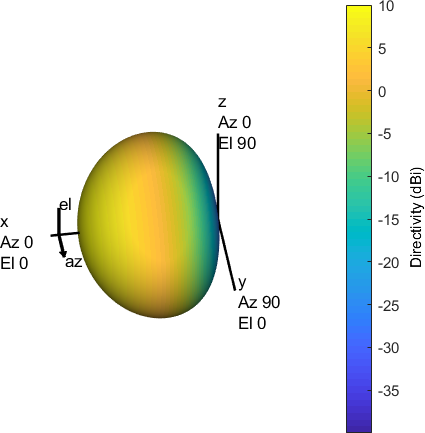
\includegraphics[width=0.415\textwidth]{hydrophone_3d.png}}
		\hfill
		\subfigure[Azimuth cut at 
		0deg]{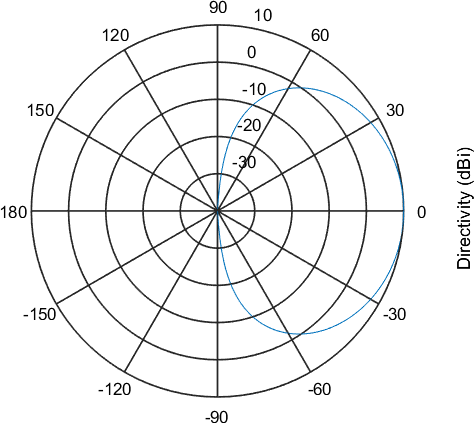
\includegraphics[width=0.45\textwidth]{hydrophone_cut.png}}
		\caption{Radiation pattern of a hydrophone element}
		\label{fig:hydrophone}
	\end{figure}
	
	Physically, hydrophones are circular, 5 cm in diameter. All hydrophones in 
	the 
	beamforming system are installed with their radiation maximum pointing to 
	zenith, i.e. perpendicular to sea surface, as described in Figure 
	\ref{fig:hydrophone}. At the other end, the ship is equipped with a single 
	hydrophone mounted on ship's hull, and pointing at nadir, i.e. 
	perpendicular to 
	seabed.
	
	Consider the signal narrowband. The ship is in the farfield of the 
	beamforming 
	system. Assume the communication link is being established in the Adriatic 
	Sea, 
	with average salinity of 38\textperthousand, and sea temperature of 20 
	\textdegree C.
	
	\subsection{Linear array}
	
	Design a single linear antenna array along the y-axis to achieve the best 
	link 
	between the habitat and the ship in four given scenarios.
	\begin{description}
		\item[Scenario 1] The ship is directly above the beamforming system.
		\item[Scenario 2] The ship is located along the longitudinal (y) axis 
		of 
		the beamforming system, at an azimuth of 30\textdegree.
		\item[Scenario 3] The ship is located along the longitudinal (y) axis 
		of 
		the beamforming system, at an azimuth of 60\textdegree.
		\item[Scenario 4] The ship is located along the longitudinal (y) axis 
		of 
		the beamforming system, at an azimuth of 70\textdegree.
	\end{description}
	
	\begin{figure}[h!]
		\centering
		\subfigure[Scenario 
		1]{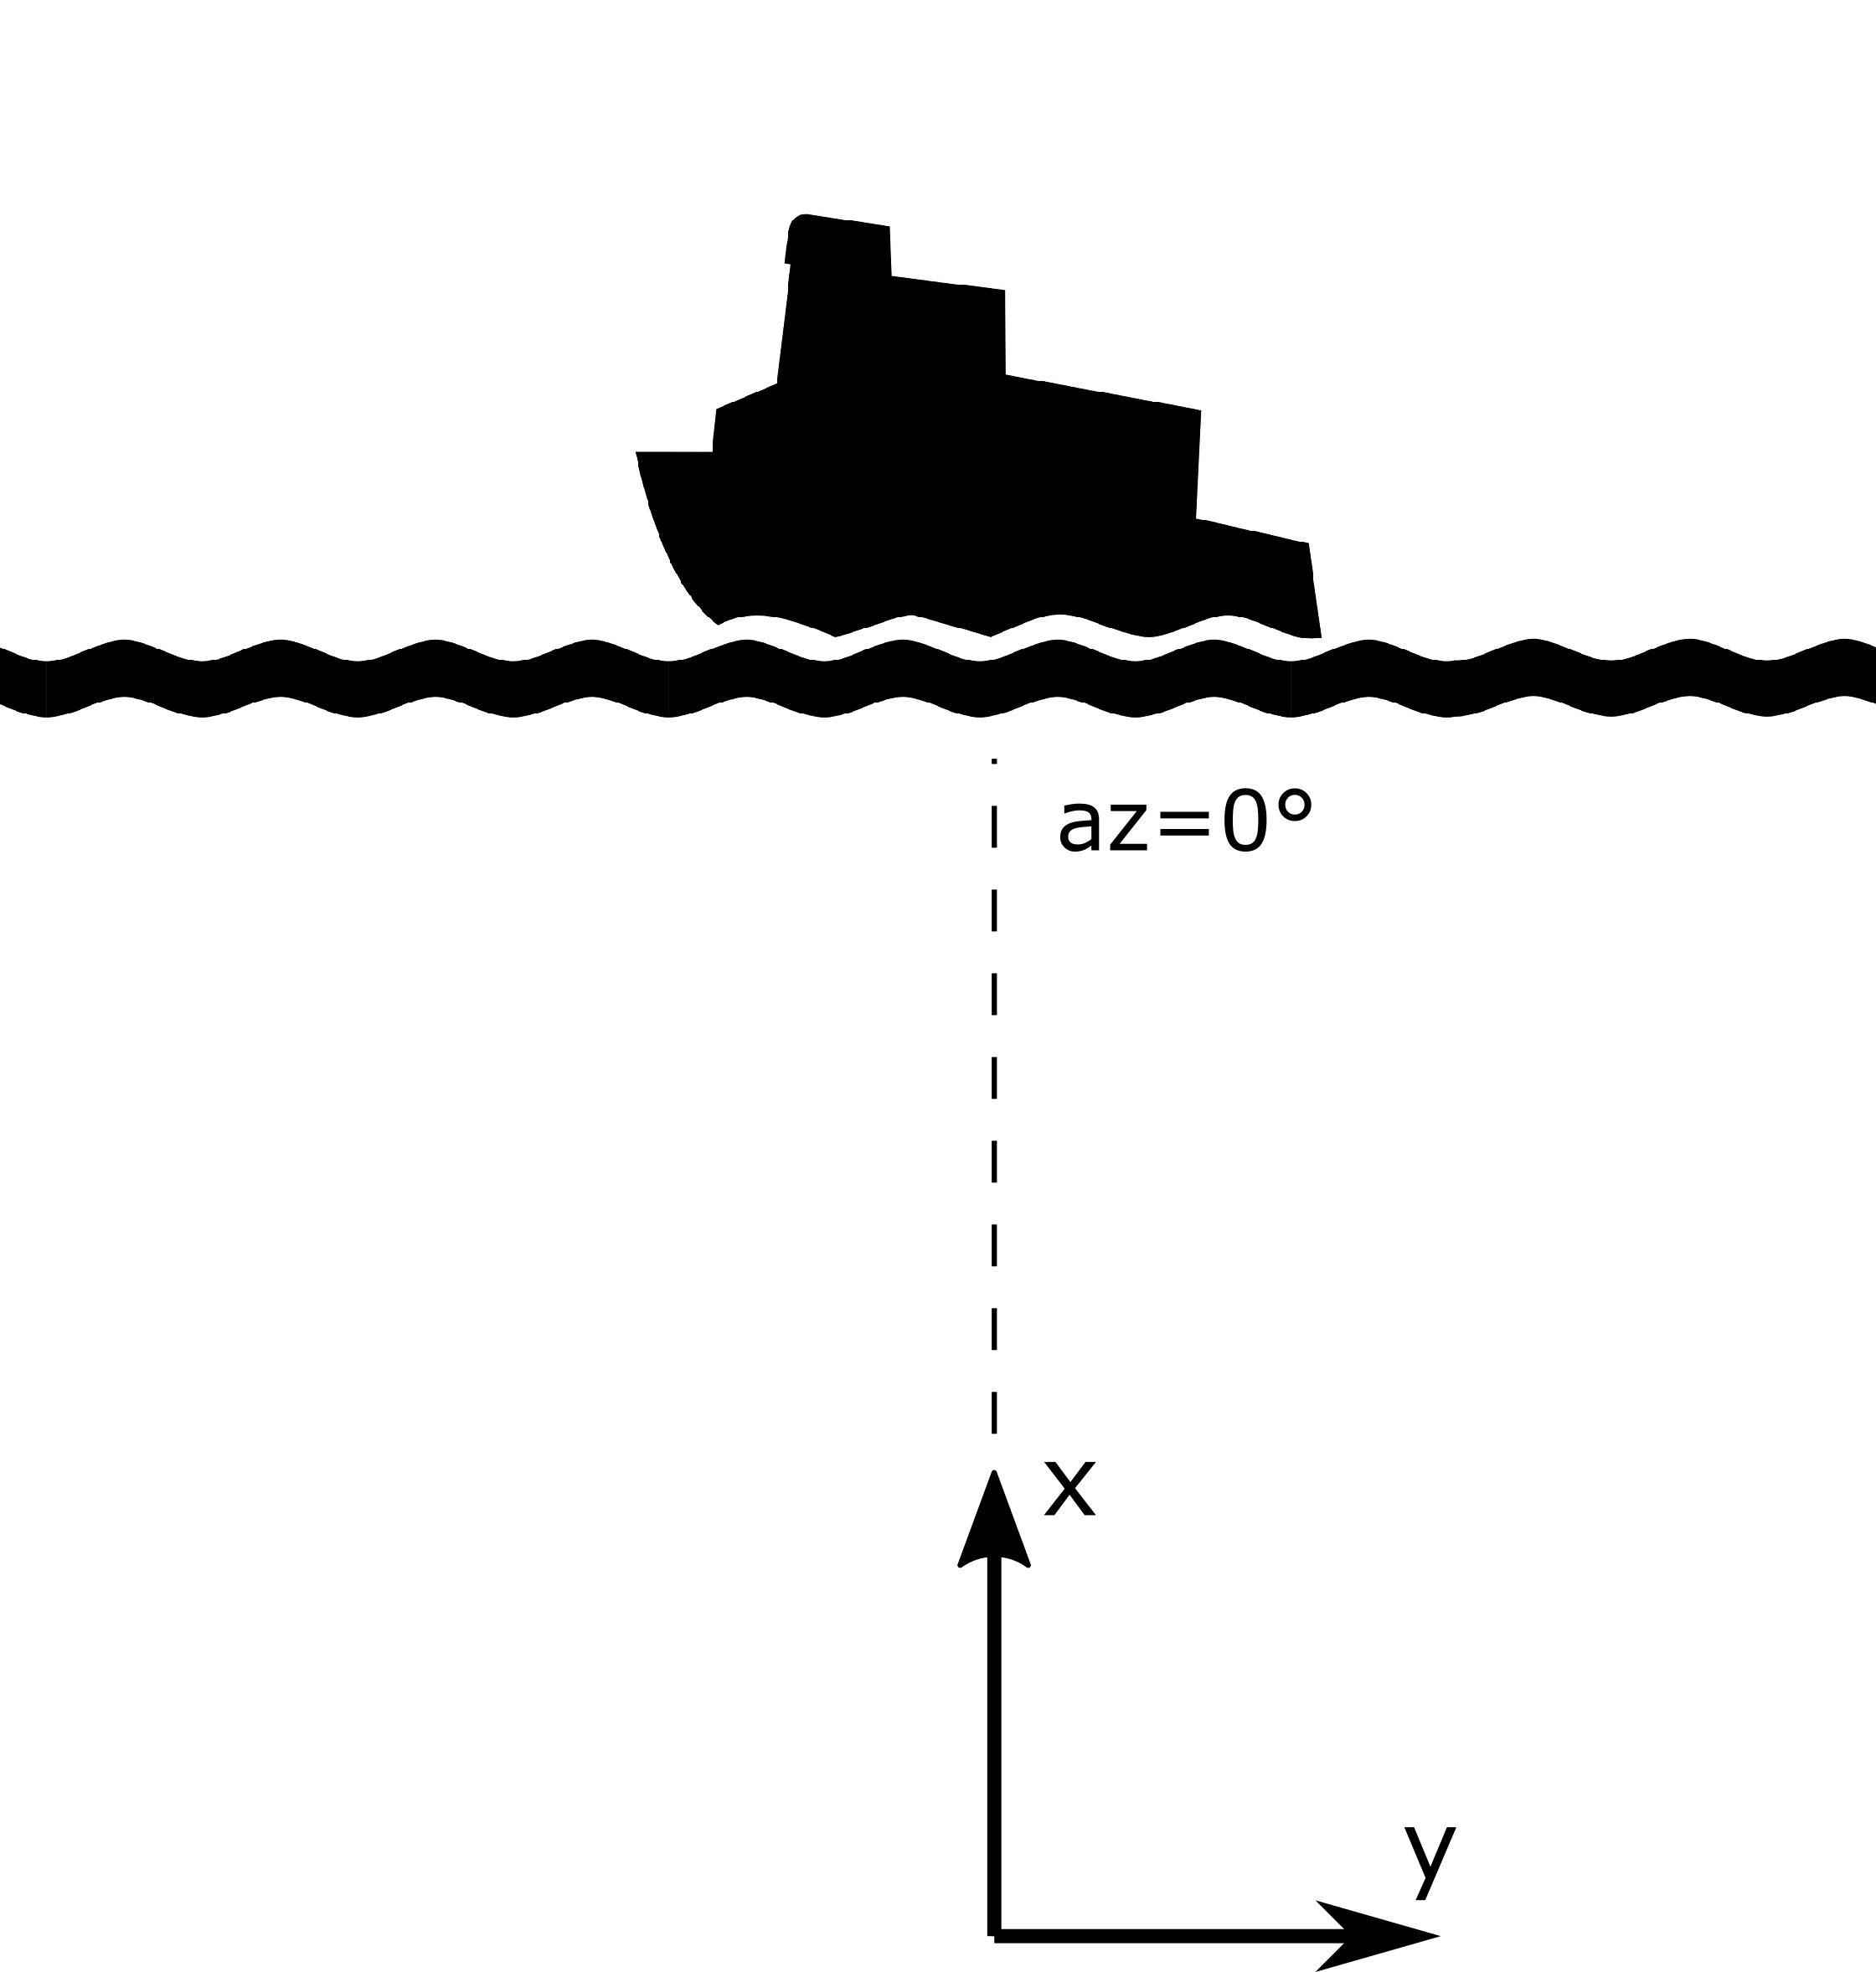
\includegraphics[width=0.45\textwidth]{scenario1.png}}
		\hfill
		\subfigure[Scenario 
		2]{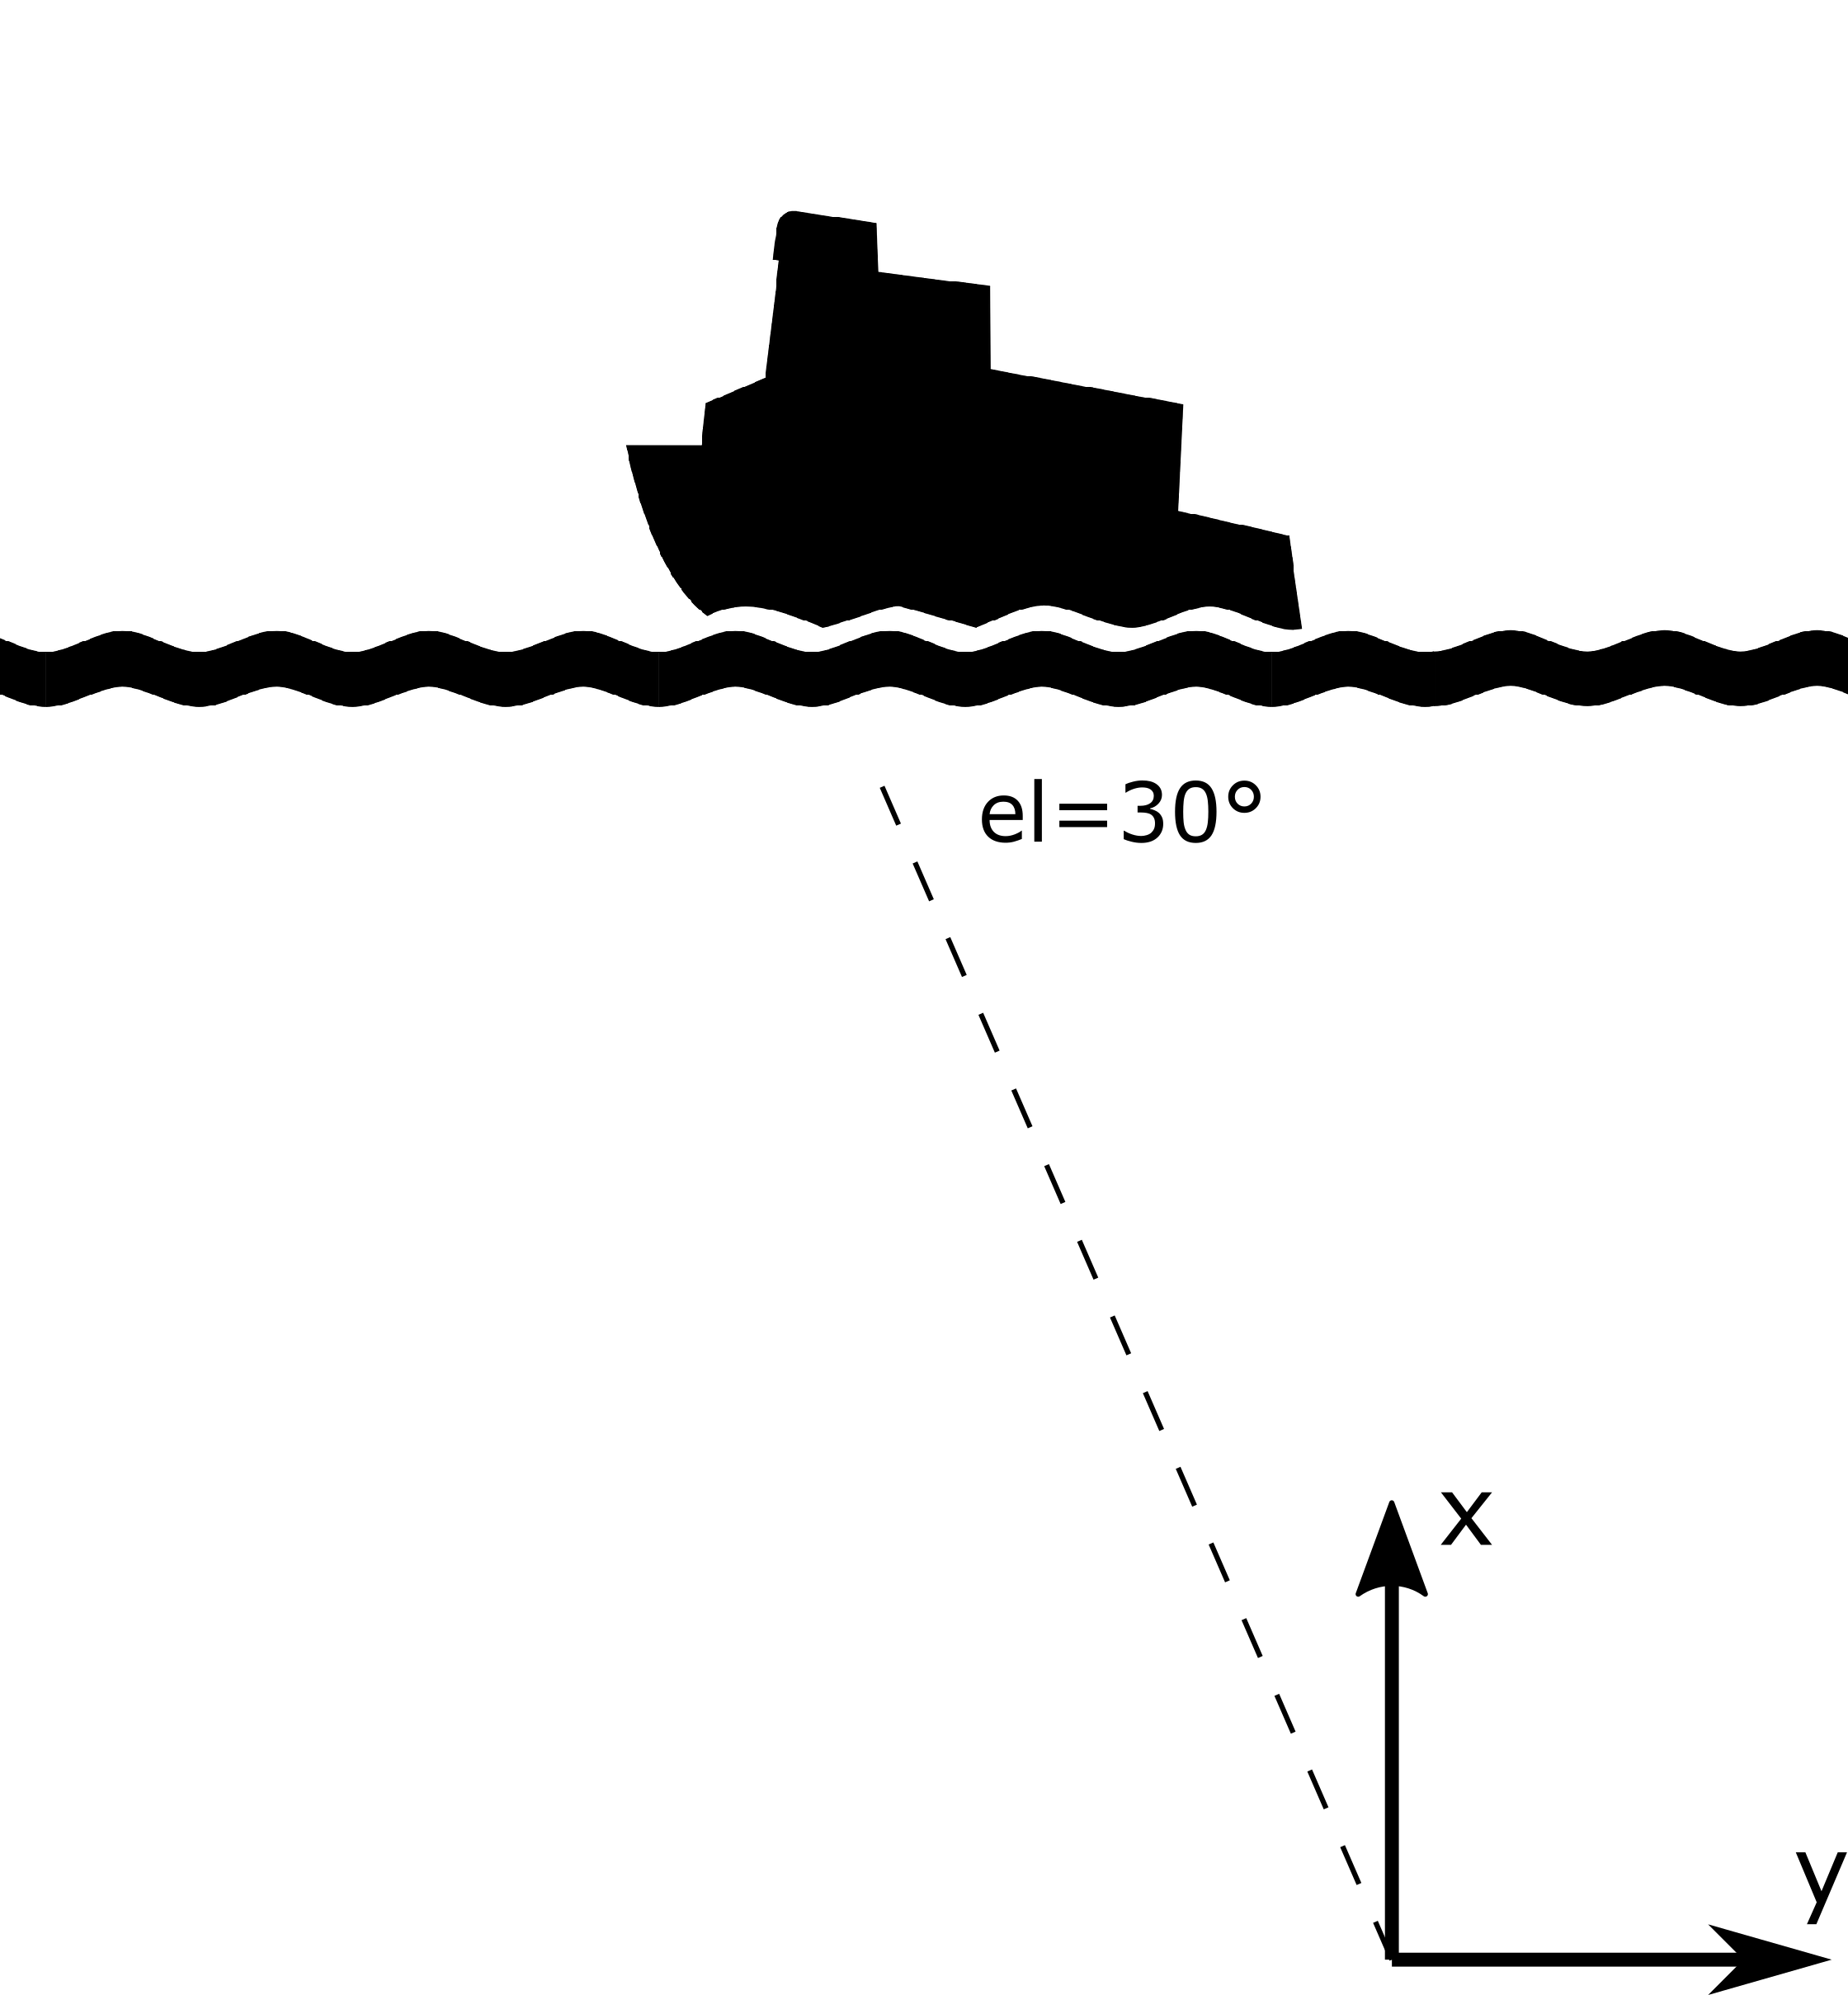
\includegraphics[width=0.45\textwidth]{scenario2.png}}
		\\
		\subfigure[Scenario 
		3]{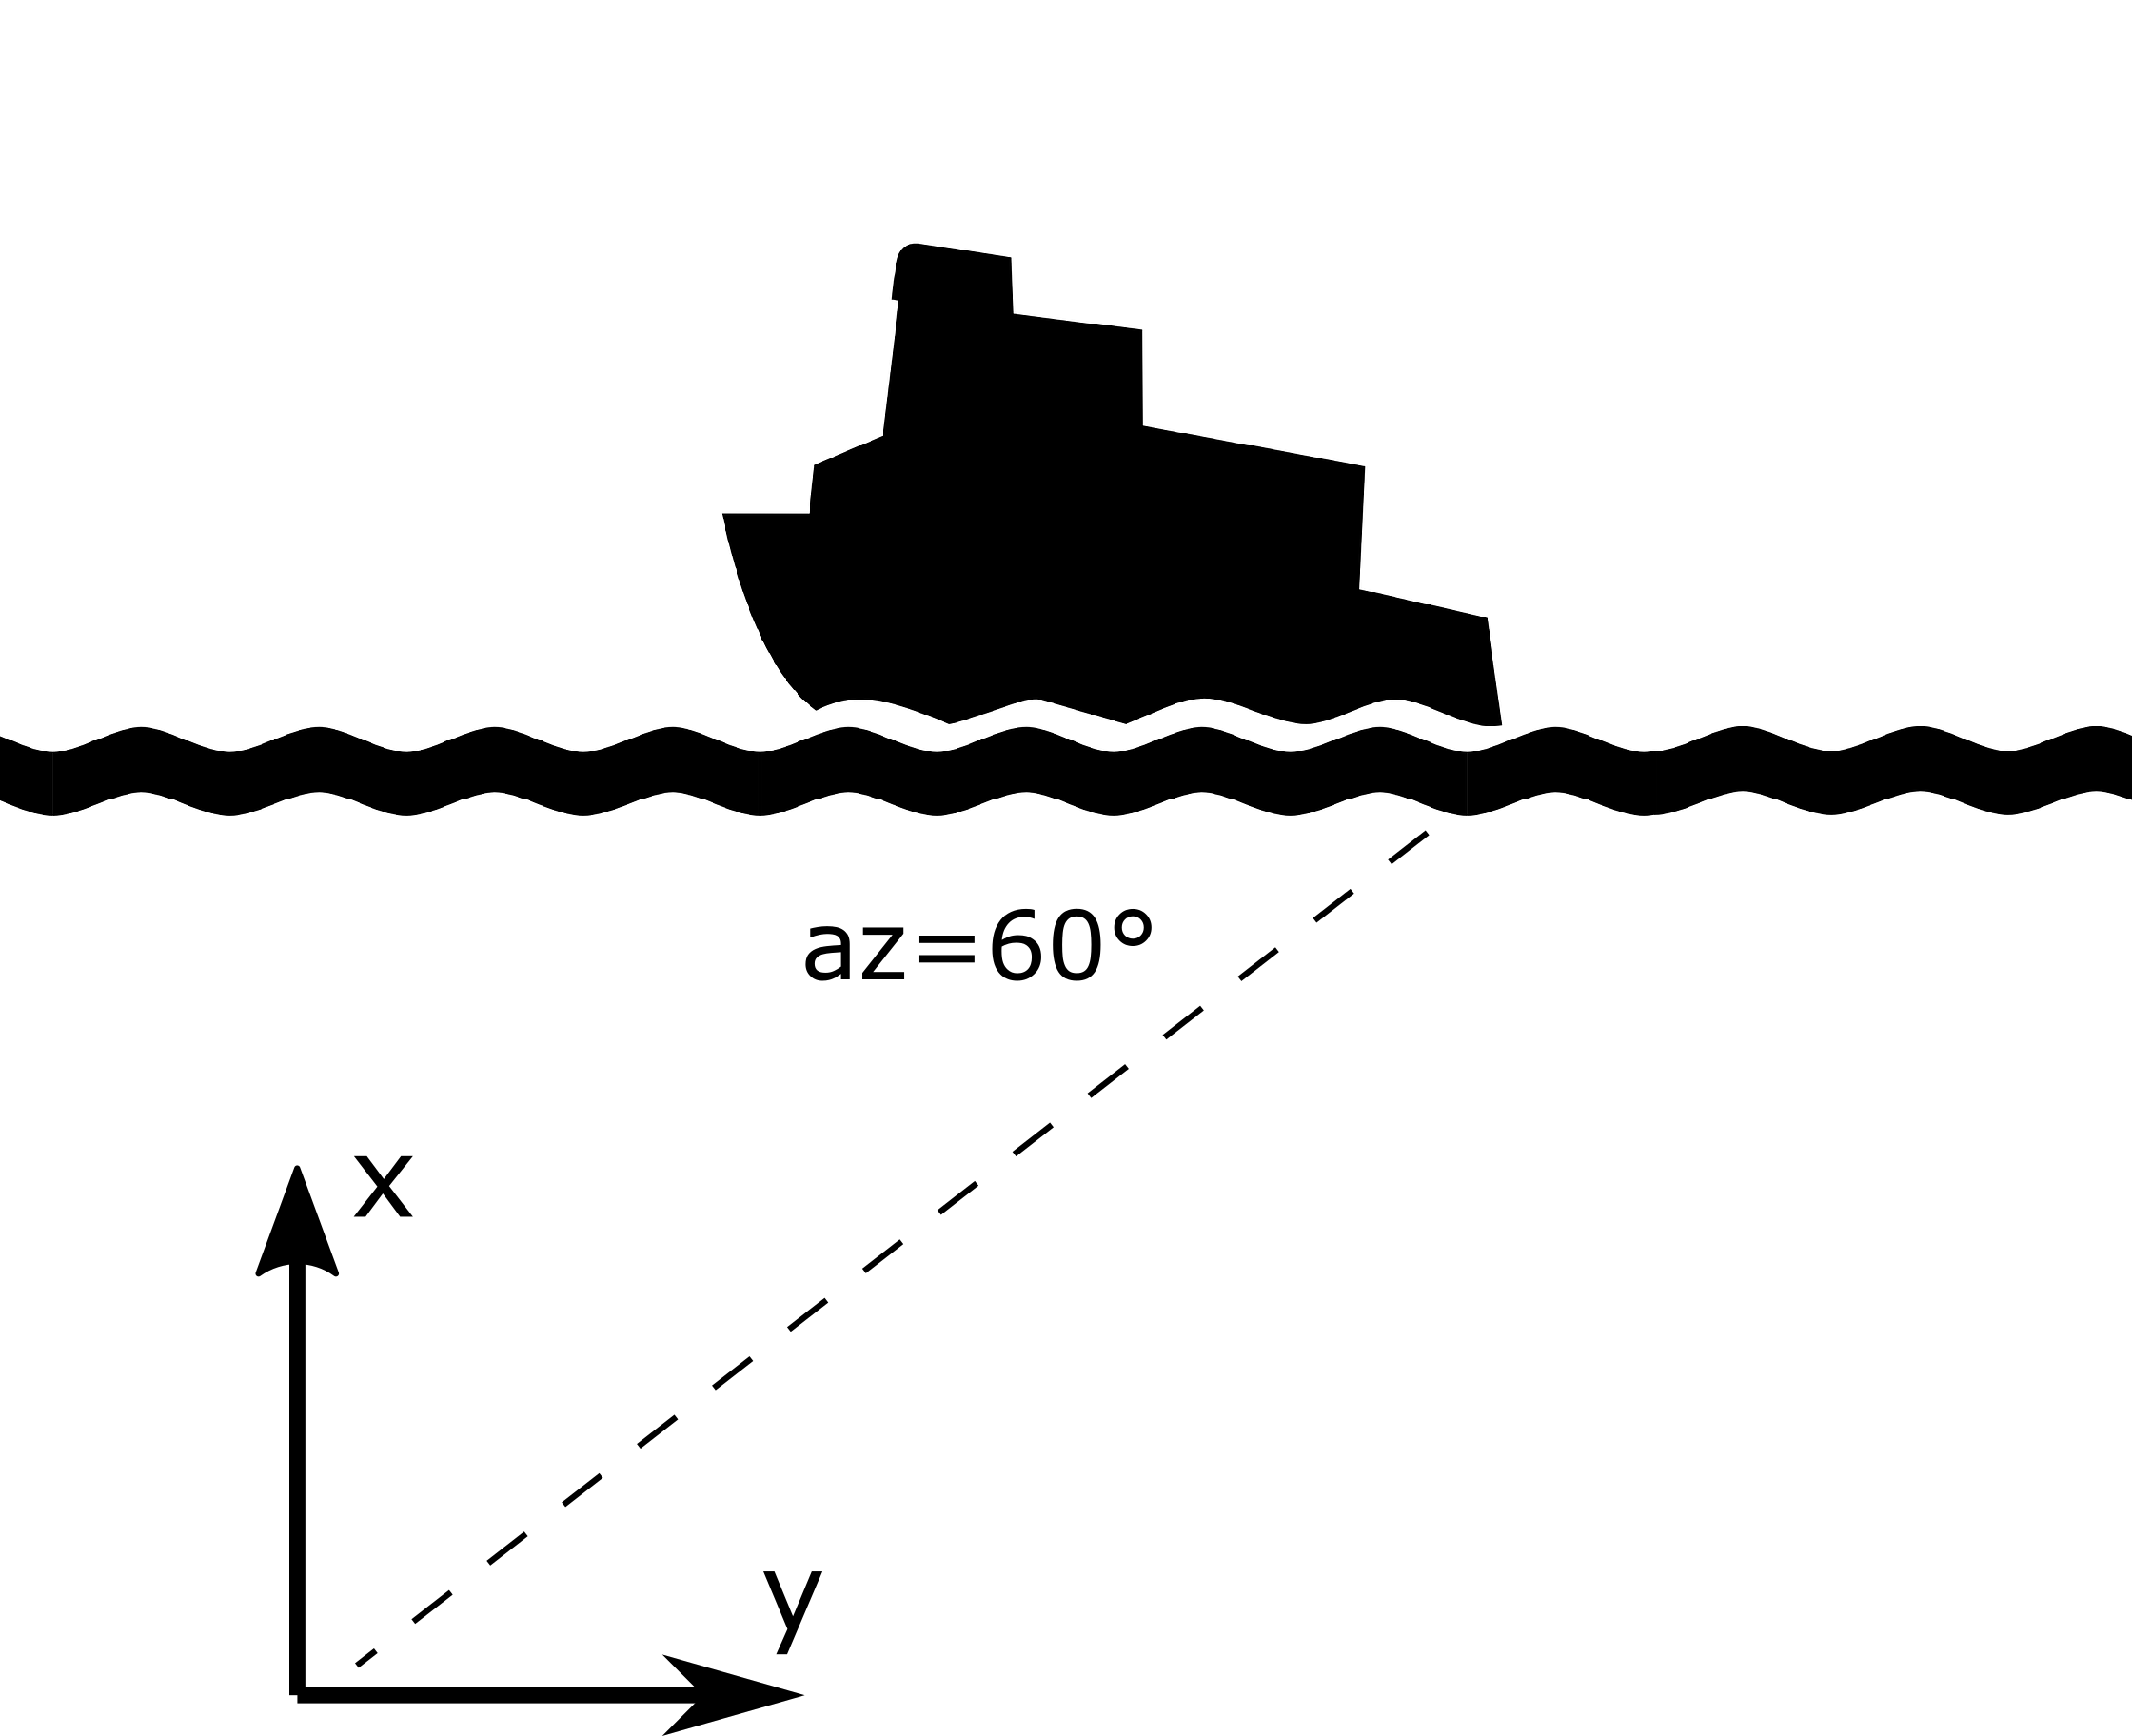
\includegraphics[width=0.45\textwidth]{scenario3.png}}
		\hfill
		\subfigure[Scenario 
		4]{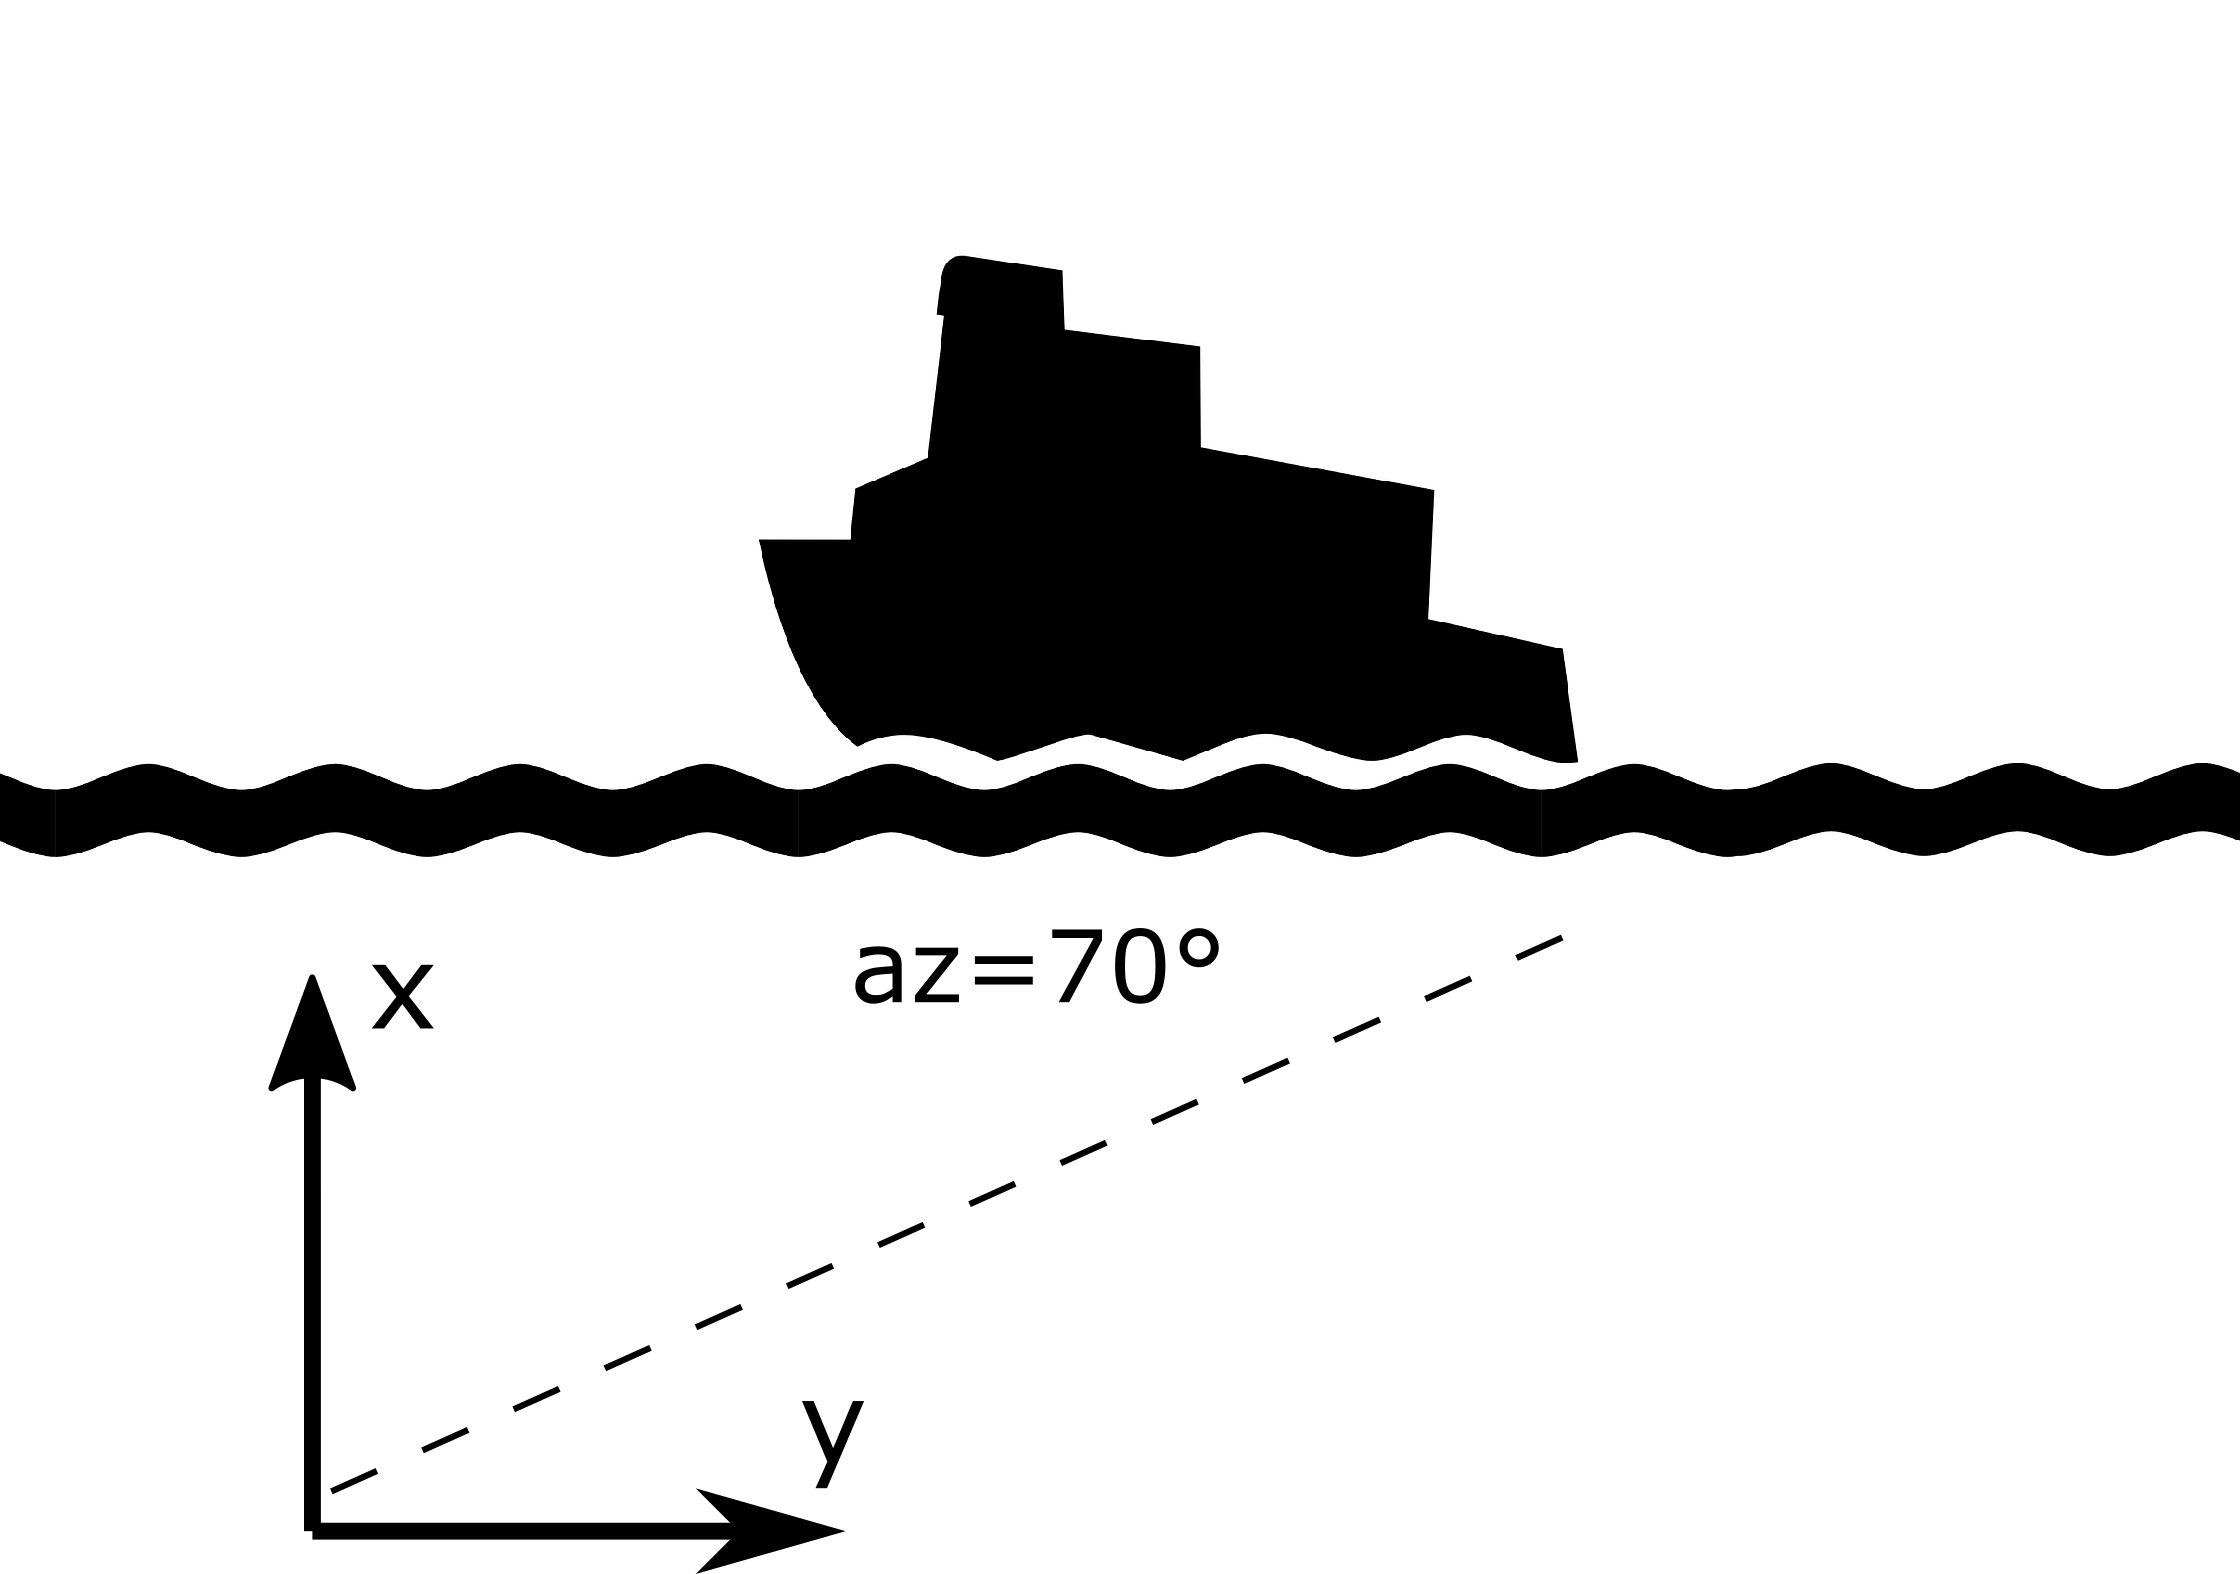
\includegraphics[width=0.45\textwidth]{scenario4.png}}
		\caption{Scenarios for Task 1}
	\end{figure}
	
	A beamforming system is defined by y coordinates of each hydrophone 
	element. 
	Number of elements is arbitrary, given the limitations introduced in 
	Introduction. The same beamforming system is used for all four scenarios. 
	For 
	each of the four scenarios, provide complex weights that are applied to 
	each of 
	the hydrophone elements to achieve optimal beamforming for the particular 
	scenario.
	
	\subsubsection*{Output data}
	
	\begin{description}
		\item[elements1.csv] \leavevmode \,\\ The file contains a one-dimensional array 
		representing the position of each hydrophone element along the y axis 
		in 
		metres.
		
		\item[scenarioX.csv] \textit{e.g. scenario1.csv, \ldots}\,\\ The file 
		contains a one-dimensional array of complex numbers representing the 
		weights applied to each hydrophone element. Weights are given for 
		elements 
		in the same order as they are listed in \textsf{elements1.csv}. Array 
		length is equal to the number of elements in the beamforming system. 
		All 
		numbers are inside, or at the edge of the unit circle.
		
		Complex numbers should be stored either in
		\begin{itemize}
			\item cartesian notation: \textsf{a+bi}, or
			\item polar notation: \textsf{P*exp(Ri)}
		\end{itemize}
	\end{description}
	
	
	\subsubsection*{Scoring}
	
	The beamforming system you designed is evaluated for each of the given 
	scenarios. For the first three scenarios, points are awarded for the 
	directivity the beamforming system achieves in the direction of the ship, 
	after 
	applying the given beamforming weights. If the ship is in the main lobe of 
	the 
	beamforming system, the number of awarded points is equal to
	\[ D_\textrm{target} - \varDelta \phi \]
	where $D_\textrm{target}$ is the directivity in the direction of the ship 
	in 
	dBi, and $\varDelta \phi$ the angular distance between the ship and the 
	direction of beamformer's maximum directivity in degrees. If the ship is 
	within 
	the strongest sidelobe of the beamforming system, the number of awarded 
	points 
	is equal to
	\[ D_\textrm{target} - \dfrac{\varDelta \phi}{10} \]
	The ship is considered to be within a radiation lobe if it is within 6 dB 
	of 
	the considered radiation lobe's maximum radiation.
	
	In scenario 4, the beamforming system is evaluated with the given 
	beamforming 
	weights, and its directivity compared to that of the same beamforming 
	system 
	with uniform excitation. The points are then awarded as
	\[ D_\textrm{target,weighted} - D_\textrm{target,uniform} \]
	The highest number of points for this scenario is 20.
	
	For all scenarios, the following rules apply: A beamforming system 
	constructed 
	with just one element is awarded no points. A beamforming system acheiving 
	negative directivity (in dBi) in the direction of the ship is awarded no 
	points.
	
	\subsection{Planar array}
	
	You will now design a planar beamforming system, to enable beamforming 
	toward a 
	ship that is moving in both dimension along the sea surface. You are given 
	a 
	single scenario (\textit{Scenario 5}) in which the ship is located at an 
	azimuth angle of 45\textdegree and at elevation of 60\textdegree, as seen 
	from 
	the reference coordinate system.
	
	\subsubsection*{Output data}
	
	\begin{description}
		\item[elements2.csv] \leavevmode \,\\ The file contains 2D coordinates of 
		beamforming 
		elements. One row of the file represents one beamforming element. The 
		first 
		column is the y-coordinate, and the second column is the z-coordinate.
		
		\item[scenario5.csv] \leavevmode \,\\ The file contains a one-dimensional array of 
		complex numbers representing the weights applied to each hydrophone 
		element. Weights are given for elements in the same order as they are 
		listed in \textsf{elements2.csv}. Array length is equal to the number 
		of 
		elements in the beamforming system. All numbers are inside, or at the 
		edge 
		of the unit circle.
		
		Complex numbers should be stored either in
		\begin{itemize}
			\item cartesian notation: \textsf{a+bi}, or
			\item polar notation: \textsf{P*exp(Ri)}
		\end{itemize}
	\end{description}
	
	\subsubsection*{Scoring}
	
	The team will achieve points that correspond to directivity in dBi in the 
	direction of the ship.
	
	A beamforming system constructed with just one element is awarded no 
	points. A 
	beamforming system acheiving negative directivity (in dBi) in the direction 
	of 
	the ship is awarded no points.
	
	\subsection{Evaluation and results}
	
	Evaluations are performed automatically, and will run continuously during 
	the 
	competition day. You can see the results of evaluation for all teams on a 
	scoring board, and thus monitor how everyone progresses. The scoring board 
	can 
	be found on \url{https://engineering.stemgames.hr}.
	
	You submit your output files to your team's Google Drive folder.
	After the simulation for your beamformer design is complete, you will find 
	evaluator's log file on Google Drive.
	
	The input files found on Google Drive at the end of the competition day 
	will be 
	taken as team's final solution. No changes will be accepted after that time.
	
	At the end of the competition day, and after the final evaluations 
	complete, 
	the total number of points awarded to the team will be normalized to the 
	best 
	team. Hence, the best team will receive 10 points, and the points received 
	by 
	other teams will be linearly scaled to the best team.
	
	
	\chapter{Day 3}
	\section{Introduction}
	
	Hello contestants!
	
	Today you will continue the work on the communication system and on the 
	next 
	stage of the power system - the power generator connected to the steam 
	turbine.
	
	
	No modern system can work without the reliable communication with the 
	outside 
	world. Today trough the solving of the SDR (Software Defined Radio) task 
	you 
	will get the feeling of what is needed to create a reliable communication 
	system.
	Once the signal has been directed using the beamforming, you need to 
	receive 
	the data being transmitted, demodulate the data and check for any errors.
	
	In most submarines, the main turbine isn't connected directly to the shaft, 
	but 
	rather to the electric generator, which charges the batteries.
	Batteries power the life support, air condition, lights, the propeller 
	motor 
	and 
	all te other submarine subsystems. 
	In continuation of the yesterdays design of the steam turbine, you will 
	have to 
	design an appropriate synchronous generator. 
	
	
	\section{Software Defined Radio}
	
	\subsection{Task 1}
	An underwater habitat controls a remotely-operated submarine by sending the 
	coordinates that the submarine has to traverse in sequence. The information 
	is modulated on top of an ultrasonic carrier, and then sent and received by 
	a hydrophone system.
	
	The 3-dimensional coordinates are organized into triplets, as 
	\textsf{xxx.xxx,yyy.yyy,zzz.zzz;} . Each digit and separating characters 
	("\textsf{,}" and "\textsf{;}") are encoded as an 8-bit ASCII character. 
	Triplets are concatenated and sent sequentially. This datastream is the 
	input to the modulating system of the transmitter.
	
	
	The transmitter first organizes the input stream into packets. Each packet 
	consists of a preamble, header, data, CRC-16 hash, and a postamble. The 
	frame structure is illustrated in Figure \ref{fig:packet}.
	
	\begin{figure}[h!]
		\centering
		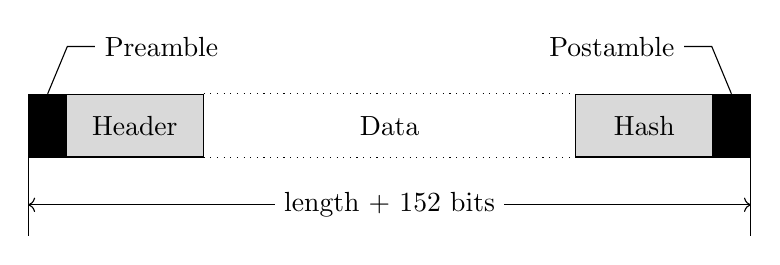
\begin{tikzpicture}[node distance=-\pgflinewidth]
		
		\node[short,fill=black] (preamb) {};
		\node[long,right=of preamb,label=center:Header](header){};
		\node[verylong,draw=none,fill=none,right=of header,label=center:Data] 
		(data) {};
		\node[long,right=of data,label=center:Hash] (hash) {};
		\node[short,fill=black,right=of hash] (postamb) {};
		
		\node[above right=0.5cm of preamb] (ppre) {Preamble};
		\node[above left=0.5cm of postamb] (ppos) {Postamble};
		
		\draw (ppre.west) -- +(-10pt,0pt) -- (preamb.north);
		\draw (ppos.east) -- +(10pt,0pt) -- (postamb.north);
		\draw[dotted] (header.north east) -- (hash.north west);
		\draw[dotted] (header.south east) -- (hash.south west);
		\draw[<->] ( $ (preamb.south west) +(0,-0.6cm) $ ) -- node[fill=white] 
		{length + 152 bits} ( $ (postamb.south east) +(0,-0.6cm) $ );
		\draw (preamb.south west) -- +(0,-1cm);
		\draw (postamb.south east) -- +(0,-1cm);
		
		\end{tikzpicture}
		\caption{Packet structure}
		\label{fig:packet}
	\end{figure}
	
	Preamble is a predefined 64-bit sequence \textsf{0xa5a5a5a5a5a5a5a5}. 
	Postamble is a bitwise-inverse of the preamble. Header is an 8-bit word 
	containing byte-length of the data section in the packet. The shortest size 
	of the data section is 64 bits, while the largest is 248 bits. The data 
	section is always byte-aligned; i.e. its length is always a multiple of 8 
	bits.
	
	All the words in the packets are stored in big endian notation. The packets 
	are sent further through the transmitter chain sequentially, without a 
	guard interval.
	
	The binary sequence of the generated packets is brought to a QPSK 
	modulator. Its constellation is represented by Figure \ref{fig:qpsk}.
	
	\begin{figure}[h!]
		\centering
		\begin{tikzpicture}
		\begin{axis}[
		xmin=-1.5,xmax=1.5,
		ymin=-1.5,ymax=1.5,
		axis lines=center,
		xlabel=$\Re e$,
		ylabel=$\Im m$,
		xtick={-1,...,1},
		ytick={-1,...,1},
		]
		\addplot+ [nodes near coords, only marks, point meta=explicit symbolic]
		table[meta=label]{
			x	y	label
			1	1	00
			-1	1	01
			-1	-1	11
			1	-1	10
		};
		\end{axis}
		\end{tikzpicture}
		\caption{QPSK modulator constellation}
		\label{fig:qpsk}
	\end{figure}
	
	The QPSK-modulated symbols are transposed to carrier frequency $f_c = 36 
	\,\textrm{kHz}$ and transmitted by a hydrophone. Transmitter data-rate is 
	9.6 kbaud. At the receiving end, the receiver aboard a submarine is 
	depicted by a block diagram in Figure \ref{fig:task1}.
	
	\begin{figure}[h!]
		\centering
		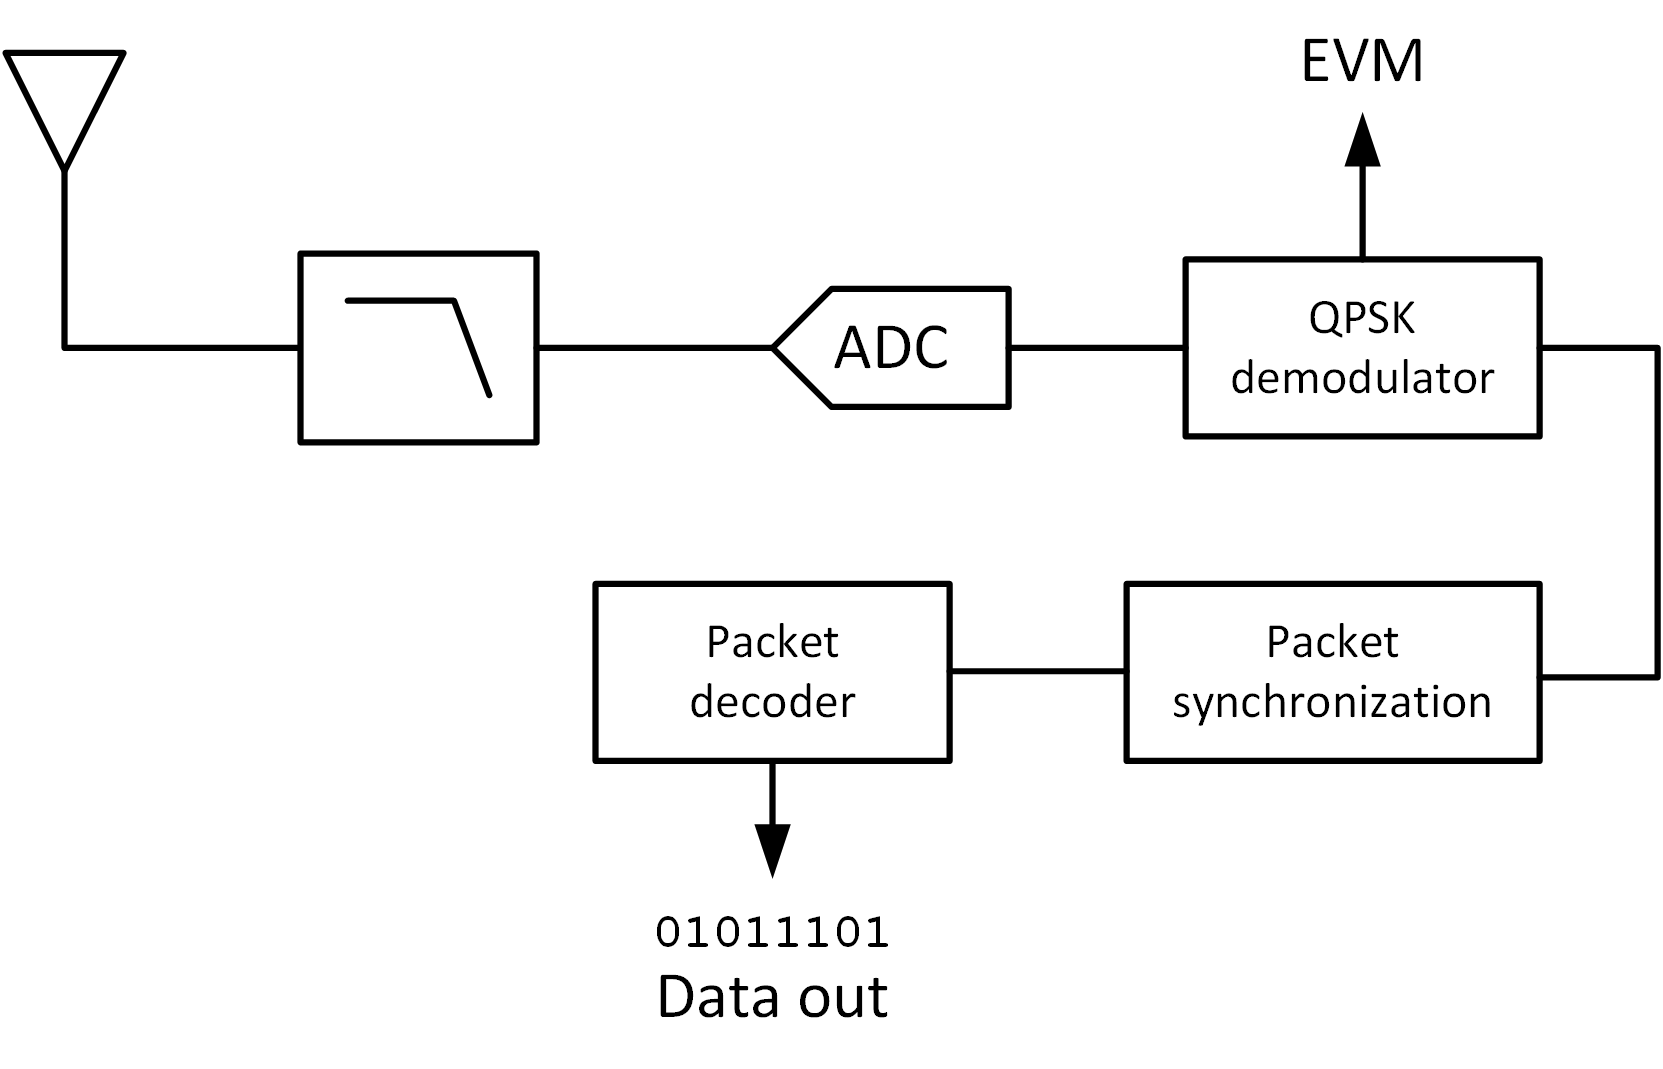
\includegraphics[width=0.9\textwidth]{Images/Task1.png}
		\caption{Receiver diagram in Task 1}
		\label{fig:task1}
	\end{figure}
	
	The ADC of the receiving hydrophone operates at a sampling frequency of 192 
	kSps. An ideal low-pass filter has a cut-off frequency of 96 kHz.
	
	You are required to implement the digital processing system of the 
	receiver, to demodulate and decode information from the received ultrasonic 
	signal.
	
	\subsubsection{Input data}
	The \textsf{single\_carrier.raw} file is given. It contains the digitized 
	signal from the ADC, recorded in 16-bit 2's complement format.
	
	\subsubsection{Implementation}
	Your solution is a C or C++ code implementing the receiver's digital 
	processing chain. Your solution consists of two files:
	\begin{description}
		\item[radio.c / cpp] Implements all the routines described further in 
		the text.
		\item[main.c / cpp] Loads the input data, calls the routines from 
		\textsf{radio.c / cpp}, and outputs decoded data to stdout in the 
		original format.
	\end{description}
	
	Your \textsf{radio.c / cpp} file must implement the following set of 
	functions:
	\begin{description}
		\item[complex *frequency\_shift(double *input, double fc, double fs, 
		int N)] \leavevmode
		\,\\ Transposes the signal provided in input from centre frequency 
		\textsf{fc} to baseband. \textsf{N} is the length of the data stream, 
		expressed as a number of double words. \textsf{fs} is the sampling 
		frequency.
		\item[double qpsk\_demodulator(complex symbol, double 
		constellation\_offset, char *decoded\_symbol)] \leavevmode
		\,\\ Decodes a baseband QPSK symbol \textsf{symbol}, and stores its 
		value to an 8-bit word \textsf{decoded\_symbol}. The function outputs 
		the EVM of the symbol.
		\item[char *bitstream\_to\_bytestream(char *bitstream, int length)] \leavevmode
		\,\\ Converts \textsf{length} 8-bits words, as output by the 
		\textsf{bitstream\_to\_bytestream} function, into a bytestream. 
		Parameter \textsf{length} is the length of the bitstream array, while 
		the length of the output array is equal to \textsf{length}/4. A pointer 
		to the beginning of the bytestream is returned.
		\item[void frame\_sync(char **bytestream, int length)] \leavevmode
		\,\\ Moves the pointer \textsf{*bytestream} to the beginning of the 
		first detected frame. \textsf{length} is the length of the bytestream.
		\item[int frame\_decoder(char *bytestream, char **data)] \leavevmode
		\,\\ Decodes the data from a single frame that starts at the pointer 
		\textsf{*bytestream}. The decoded data should be stored to 
		\textsf{*data}. The return value is the length of processed data (frame 
		length).
	\end{description}
	
	You are provided with some helper files:
	\begin{description}
		\item[api.h] \leavevmode
		\,\\ An API containing some types, functions and constants you may find 
		useful.
		\item[api.c] \leavevmode
		\,\\ The compiled API described in \textsf{api.h}.
	\end{description}
	
	
	\subsubsection{Evaluation}
	
	You have access to an evaluation server to which you can upload your source 
	files.
	The server will execute your code and verify the functionlity of each 
	function implemented in your \textsf{radio.c / cpp} file.
	The server functionality will further be described in a document that you 
	will receive at the start of the competition day.
	
	\subsection{Task 2}
	
	Along the submarine's trajectory information, the habitat and the submarine 
	exchange location data on debris scattered around the sea. This data is 
	transmitted in a separate data stream from the trajectory coordinates, and 
	it has the same triplet format as the data from Task 1. Also, the data is 
	packaged in the same manner as in Task 1. The resulting bitstream is then 
	spread into 4 QPSK subcarriers, as depicted in Figure \ref{fig:spread}.
	\begin{figure}[h!]
		\centering
		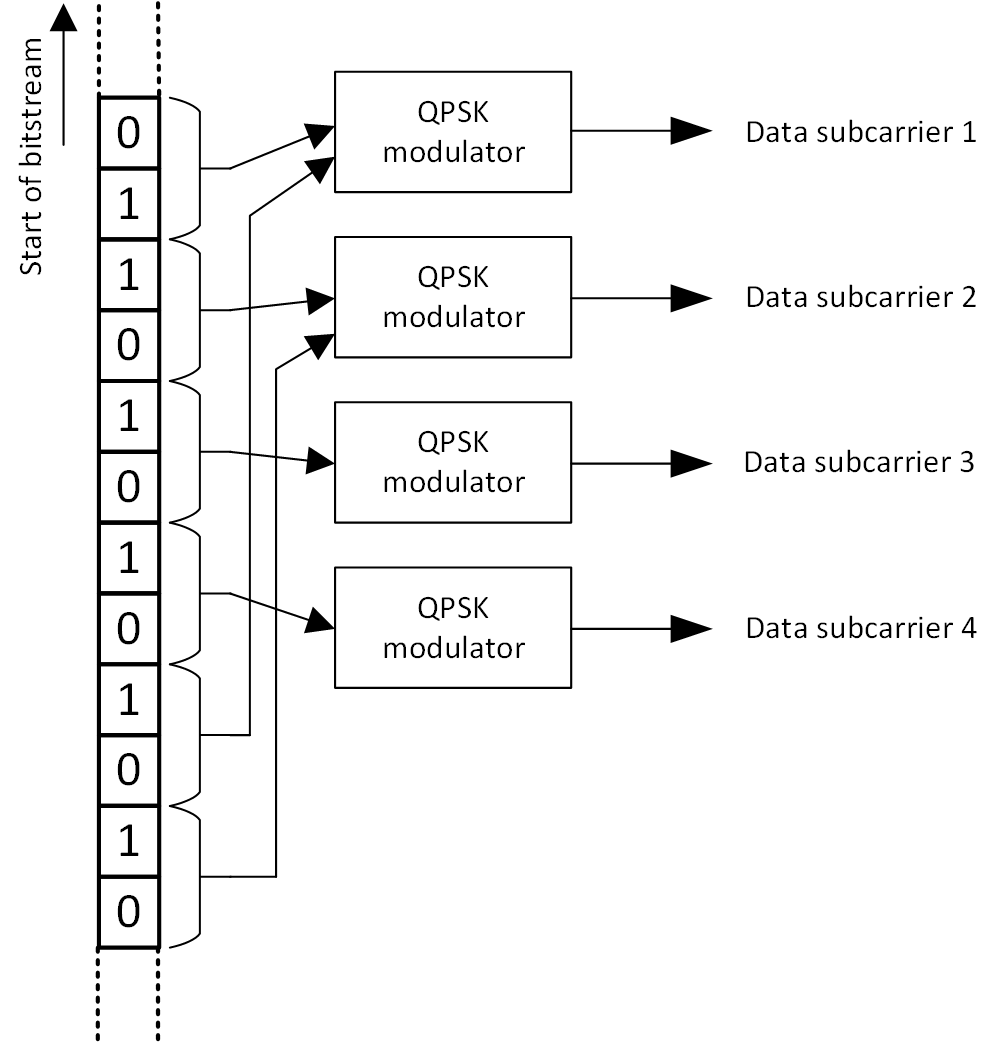
\includegraphics[width=0.7\textwidth]{Images/spread.png}
		\caption{Bitstream spreading mechanism}
		\label{fig:spread}
	\end{figure}
	
	The obtained QPSK carriers are multiplexed into OFDM that consists of a 
	total of 9 subcarriers. These are organized as depicted by DFT spectrum in 
	Figure \ref{fig:dft}.
	\begin{figure}[h!]
		\centering
		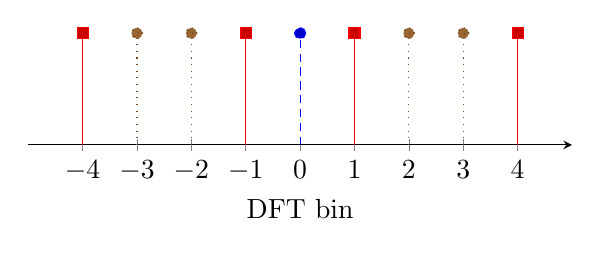
\begin{tikzpicture}
		\begin{axis}[
		width=0.7\textwidth,
		height=3cm,
		axis x line=bottom,
		axis y line=none,
		xlabel=DFT bin,
		ymin=0,ymax=1,
		xmin=-5,xmax=5,
		xtick={-4,...,4}
		]
		% Osnovni podatak
		\addplot+ [ycomb, style={densely dashed}] plot coordinates {
			(0,1)
		};
		% Piloti
		\addplot+ [ycomb, style={solid}] plot coordinates {
			(-4,1) (-1,1) (1,1) (4,1)
		};
		% Ostali nosioci
		\addplot+ [ycomb, style={dotted}] plot coordinates {
			(-3,1) (-2,1)
			(2,1) (3,1)
		};
		\end{axis}
		\end{tikzpicture}
		\caption{OFDM carrier DFT spectrum}
		\label{fig:dft}
	\end{figure}
	
	Subcarrier spacing is $\varDelta f = 1500 \,\textrm{Hz}$. The graph in 
	Figure \ref{fig:dft} is centred to frequency $f_c = 36 \,\textrm{kHz}$, 
	corresponding to the central frequency of the OFDM carrier. The subcarrier 
	at bin 0, depicted by a dashed line, contains trajectory coordinate stream 
	from Task 1. Subcarriers depicted by dotted lines contain the data stream 
	added for this task. Subcarriers depicted by a solid line are pilots. OFDM 
	symbols have no cyclic prefix.
	
	The receiver code from Task 1 has to be modified to work with an OFDM 
	carrier, and decode the additional data stream. Block diagram of the 
	receiver is presented in Figure \ref{fig:task2}.
	
	\begin{figure}[h!]
		\centering
		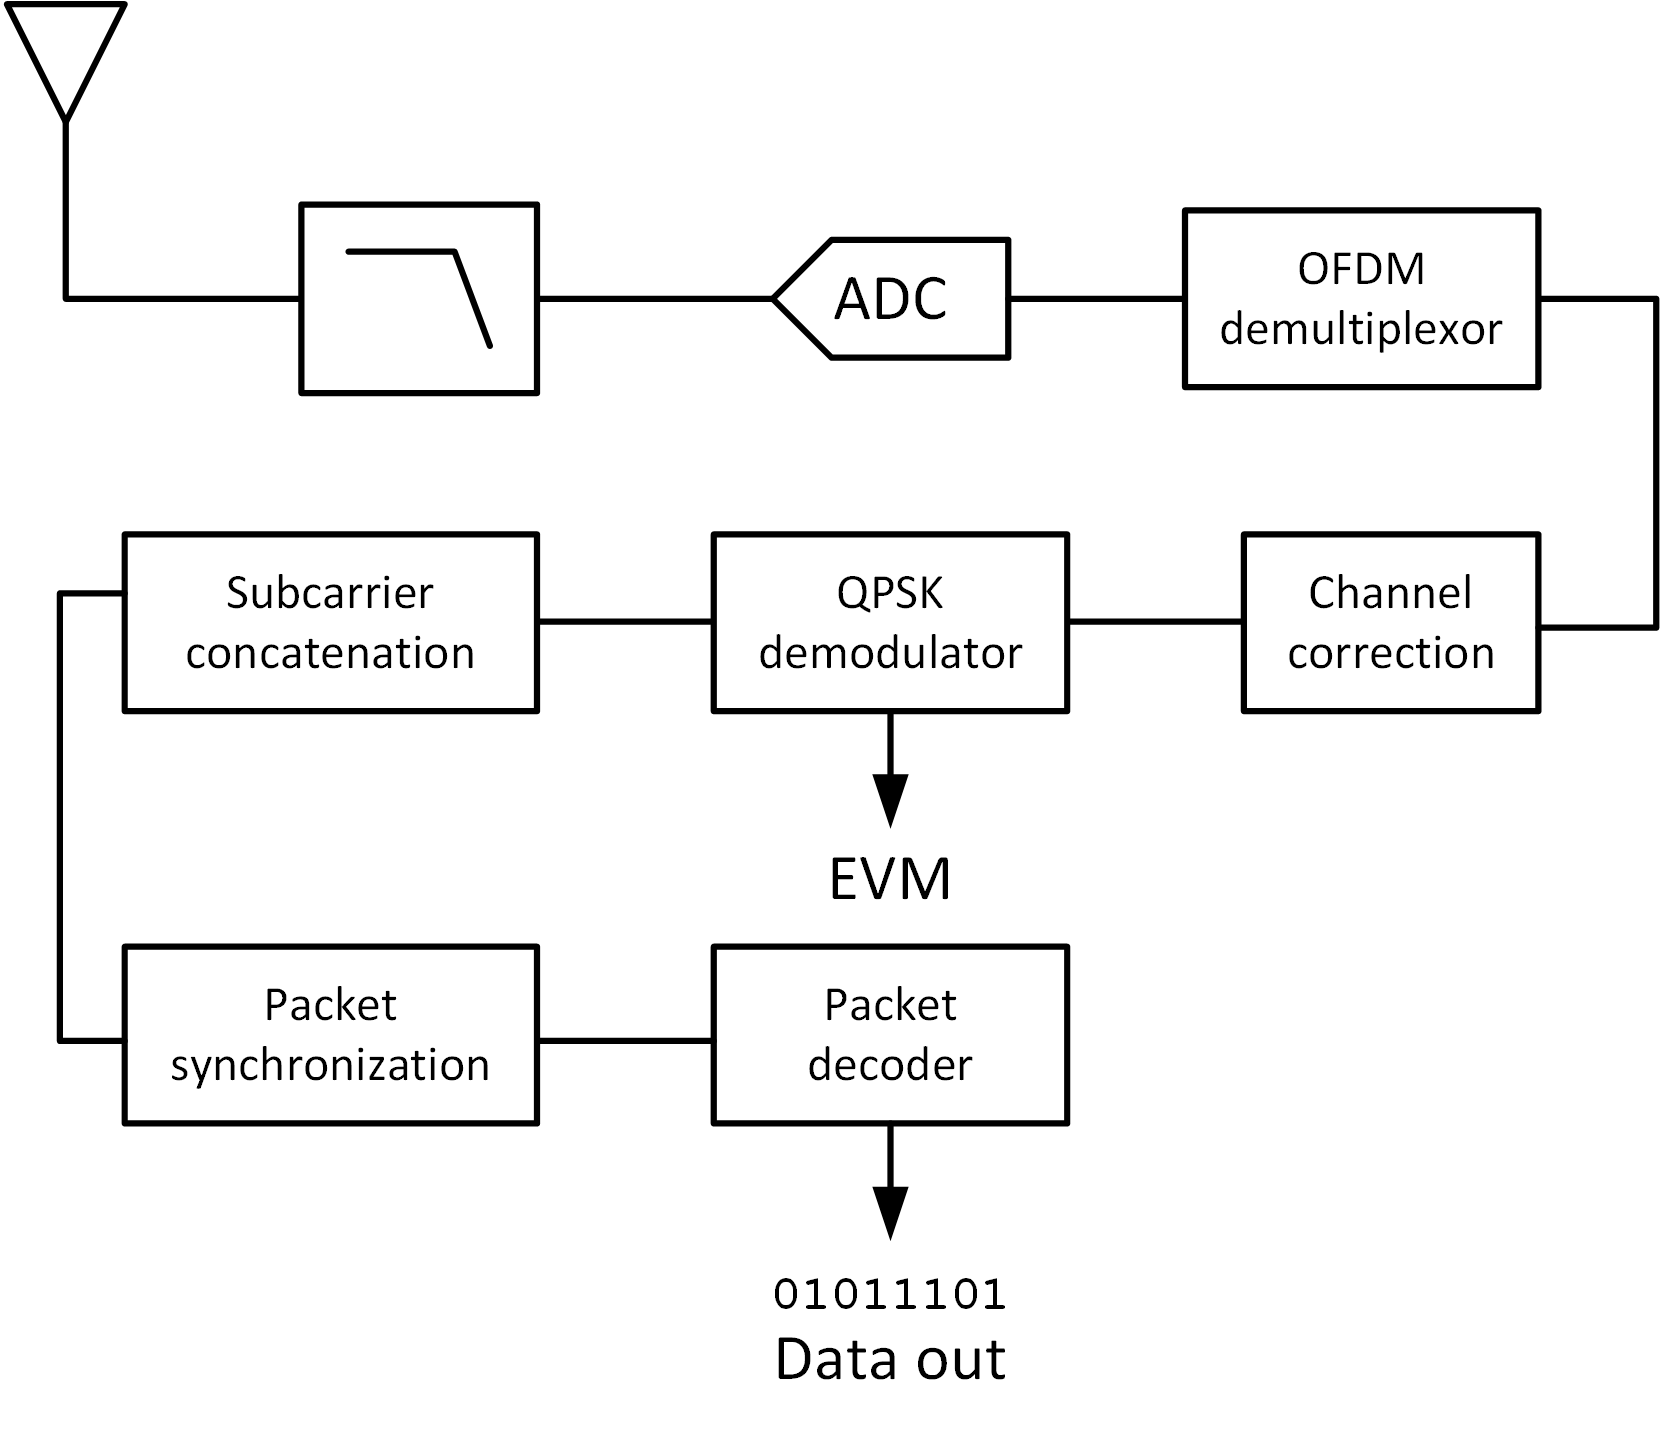
\includegraphics[width=0.9\textwidth]{Images/Task2.png}
		\caption{Receiver diagram in Task 2}
		\label{fig:task2}
	\end{figure}
	
	\subsubsection{Input data}
	The \textsf{ofdm\_carrier.raw} file is given. It contains the digitized 
	signal from the ADC, recorded in 16-bit 2's complement format.
	
	\subsubsection{Implementation}
	You should update your \textsf{radio.c / cpp} and \textsf{main.c / cpp} to 
	implement the new features required for Task 2. Your \textsf{radio.c / cpp} 
	file should implement the following additional functions:
	\begin{description}
		\item[double *ofdm\_demodulator(complex *spectrum, int *carrier\_idx, 
		int carrier\_no, char **data)] \leavevmode
		\,\\ Takes the spectrum of a \underline{single OFDM symbol} from 
		\textsf{*spectrum}, and demultiplexes the subcarriers containing the 
		\underline{additional data stream}. The demodulated QPSK symbols from 
		these subcarriers are stored in a bitstream array that starts at 
		\textsf{*data}. Demodulated QPSK symbols from each subcarrier are 
		stored in their own \textsf{char}s, to be used as input to the 
		\textsf{bitstream\_to\_bytestream} function. The input signal is in 
		baseband in the original sample rate. \textsf{carrier\_idx} is a list 
		of DFT bins that contain the additional data stream. 
		\textsf{carrier\_no} is the length of \textsf{carrier\_idx} array.
	\end{description}
	
	\subsubsection{Evaluation}
	
	OFDM-capable \textsf{radio.c / cpp} file is submitted at the end of the 
	competition day.
	
	\subsection{Task 3}
	An algorithm for calculating the CRC-16 hash of an input stream should be 
	added to solutions for both tasks. CRC-16 verification should first be 
	implemented as a separate function, and then integrated into the receiver 
	chain. The modification is presented in Figure \ref{fig:task3}.
	
	\begin{figure}[h!]
		\centering
		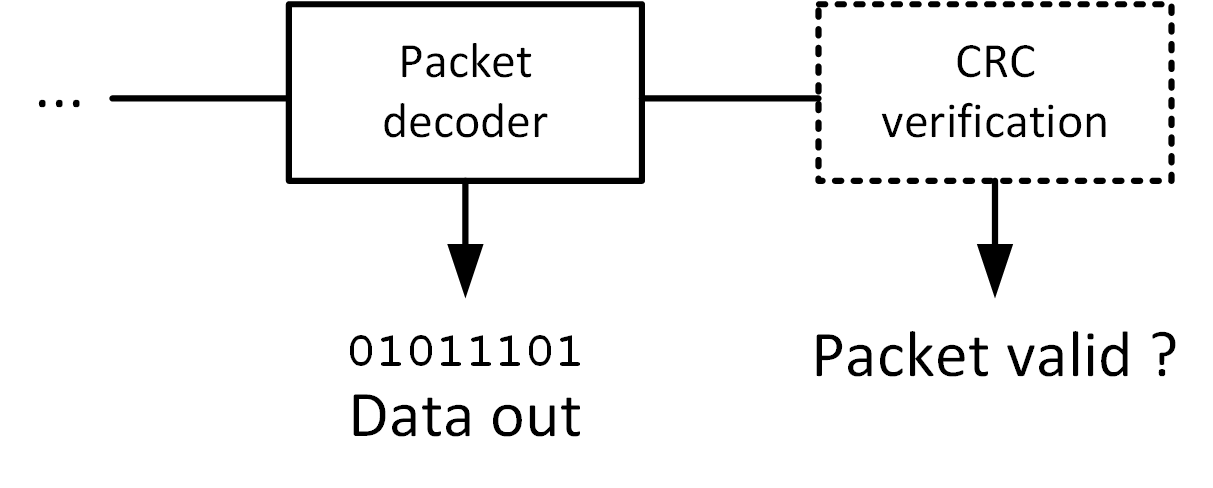
\includegraphics[width=0.7\textwidth]{Images/Task3.png}
		\caption{CRC check in receivers}
		\label{fig:task3}
	\end{figure}
	
	The CRC-16 hash in data frames is calculated using the CRC-CCITT algorithm, 
	with an initial register state \textsf{0xffff}.
	
	\subsubsection{Implementation}
	Your \textsf{radio.c / cpp} code must implement the following additional 
	functions:
	\begin{description}
		\item[char crc16\_check(char* bitstream, int length)] \leavevmode
		\,\\ Returns CRC-16 hash of the given \textsf{bitstream}, of length 
		\textsf{length}.
		\item[int frame\_decoder\_valid(char* bytestream, char** data, bool 
		*valid)] \leavevmode
		\,\\ Decodes the data from a single frame that starts at the pointer 
		\textsf{*bytestream}. The decoded data should be stored to 
		\textsf{*data}. The output flag \textsf{*valid} denotes if the decoded 
		frame has a valid CRC-16 checksum. The return value is the length of 
		processed data (frame length).
	\end{description}
	
	\subsubsection{Evaluation}
	
	A \textsf{radio.c / cpp} capable of performing error detection is submitted 
	at the end of the competition day.
	
	\subsection{Documentation}
	
	Provide documentation that describes your solution for the receiving chain. 
	Back your implementation by describing the mathematical background of your 
	processing chain. Document the datasets you used to evaluate your solution.
	
	The documentation will not be graded, but it can help mentors in 
	understanding your approach and validating the theory behind your solution.
	
	\newpage
	\section{Synchronous machine design}
	
	\subsection{Introduction}
	
	Your submarine needs electric power to drive the main propeller shaft and 
	to operate all the equipment on board. The main supply of the electric 
	power on your submarine is a synchronous generator. The generator rotor is 
	fitted on the same shaft as the steam turbine. The generator converts the 
	mechanical power from the steam turbine into electrical energy which is 
	supplied to each load on the submarine. Generators are typically purchased 
	based on the requirements of a specific application. In this task you will 
	be designing a three-phase synchronous generator for your submarine. 
	Nominal values of the synchronous generator are given as: 
	\begin{table}[h!]
		\hyphenpenalty 10000
		\caption{Nominal values of the generator}
		\label{tab:nominalValues}
		\begin{tabularx}{\textwidth}{|Y|Y|Y|Y|} \hline
			\textbf{No. of Phases} & 3 & \textbf{Frequency} & 50 Hz \\ \hline 
			\textbf{Voltage} & 400 V, {\Large $\wye$} & \textbf{Speed} & 3000 
			rpm \\ \hline
			\textbf{Power rating} & 100 kVA & \textbf{Power factor} & 80 \% \\ 
			\hline
		\end{tabularx}
	\end{table}
	
	\subsection{Calculation of the machine parameters}
	Synchronous generator design is not a simple task and to make it easier for 
	you only a limited  number of parameters needs to be determined. 
	\\The main dimensions of the generator that you need to calculate are:
	\begin{itemize}
		\item the stator bore diameter,
		\item the rotor diameter,
		%    \item the air gap length.
	\end{itemize}
	All of the machine main dimensions must be calculated in meters.
	\\Next, you have to determine:
	\begin{itemize}
		\item the number of conductors in the stator slots (round to the first 
		higher integer),
		\item the number of field winding turns (integer).
	\end{itemize} 
	Lastly, the design of the generator is finished with the calculation of the 
	synchronous reactance in p.u. 
	\\Generators used in applications with steam turbines (high-speed 
	applications) are ones with a cylindrical (round) rotor. The rotor body of 
	the generator is typically a solid piece of steel for reasons of strength, 
	given the high rotational speeds to which the rotor is subjected. The rotor 
	diameter is sized to operate at near the stress limit of the steel alloy. 
	The maximum allowable peripheral speed of the generator is $80\ 
	\mathrm{m/s}$ which means the machine must be capable of sustaining 70 \% 
	overspeed. 
	\\Windings located on the rotor of the generator are called field 
	(excitation) windings. Field windings are supplied with direct current. The 
	external source used to provide DC current is commonly referred to as an 
	exciter. At the no-load condition, the exciter supplies field windings with 
	DC current equal to $28\ \mathrm{A}$ which is required to create a field 
	current linkage of $1904\ \mathrm{A}$. In order to describe the magnetic 
	circuit of the machine and the required field current linkage, Ampere's law 
	may be used. The current linkage produces magnetic flux density 
	sinusoidally distributed along the pole. During half of the period $T$ the 
	flux density wave travels one stator pole pitch. The maximum value of the 
	magnetic flux density in the air gap is 0,8 T and the length of the air gap 
	is constant. Iron's magnetic permeability can be assumed to be infinite in 
	comparison with the magnetic permeability of air. 
	Stator windings or armature windings are full-pitch one-layer windings 
	embedded in 36 slots. Stator length is $0.5\ \mathrm{m}$. A synchronous 
	generator can be represented by a simple equivalent circuit as shown in 
	figure \ref{fig:01}. Phase voltage measured on the output terminals of the 
	generator is lower than the induced phase voltage due to the voltage drop 
	on the stator impedance. The synchronous reactance prevails in the stator 
	impedance which means that the stator resistance can be neglected when 
	calculating the synchronous reactance. In nominal conditions (nominal 
	voltage, power factor and load) the angle between the terminal voltage and 
	the induced voltage is equal to $25.07^{\circ}$.
	\begin{figure}[!htb]
		\centering
		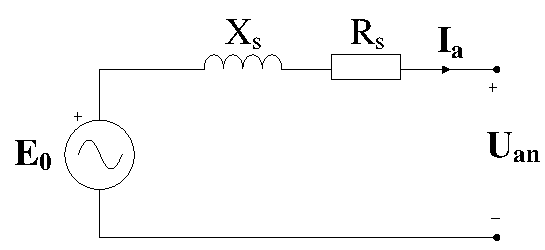
\includegraphics{Images/EquivalentCircuit.pdf}
		\caption{Synchronous machine equivalent circuit}
		\label{fig:01}
	\end{figure}
	In order to determine the characteristics of the synchronous generator 
	standardized tests must be carried out. The simplest method by which this 
	is achieved are the open-circuit and the short-circuit tests. Typical 
	open-circuit and short-circuit curves are shown in figure \ref{fig:02}. 
	During the open-circuit the field winding is supplied with the nominal 
	field current $I_{fn}$ and the line voltage measured on the generator 
	terminals is equal to $680.235\ \mathrm{V}$. In case when the field current 
	is equal to $I_{f0} = 28 \ \mathrm{A}$, the voltage measured at the 
	generator terminals will be equal to the nominal voltage. During the 
	short-circuit test when the field winding current equals to $I_{f0}$ the 
	measured stator current will be $92.524\ \mathrm{A}$.
	\\The per-unit system is widely used within the analysis of electrical 
	machines. Per-unit values are obtained by dividing each parameter by a base 
	value. For this task the base values are defined with:
	\begin{itemize}
		\item peak value of the rated stator phase voltage,
		\item rated apparent power,
		\item rated angular frequency,
		\item peak value of the rated stator phase current.
	\end{itemize}
	
	
	\begin{figure}[!htb]
		\centering
		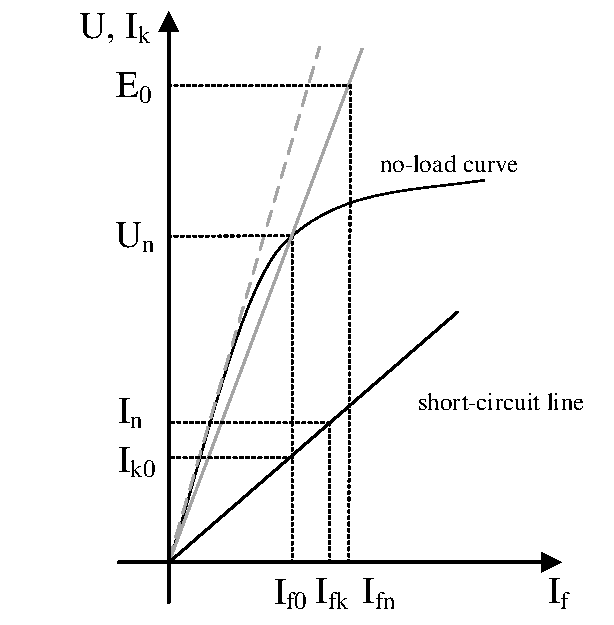
\includegraphics[scale=0.5]{Images/NoLoadCurveShortCircuit.pdf}
		\caption{Open-circuit and short-circuit curves}
		\label{fig:02}
	\end{figure}
	\newpage
	\subsection{Solution format and grading scheme}
	Your solution must be submitted as a .csv format document with only 2 rows. 
	File name must be 
	\texttt{machineParameters.csv}. The first row must consist of the required 
	parameter names and the second row of numerical values that you calculated 
	for each parameter. Column names must be marked as follows (columns should 
	be in exactly this order):
	\begin{itemize}
		\item stator bore diameter \textbf{Ds},
		\item rotor diameter \textbf{Dr},
		\item air gap length \textbf{delta},
		\item number of conductors in the stator slots \textbf{z},
		\item number of field winding turns \textbf{Nf},
		\item synchronous reactance in p.u \textbf{Xd}.
	\end{itemize}
	This task is graded up to 20 points. 3 points are given for  each correctly 
	calculated parameter and 2 points are given for the documentation. The 
	documentation is submitted at the end of the day. The documentation must 
	include your calculations along with some short comments explaining the 
	equations. You can choose the format in which the documentation will be 
	submitted (.c script, .m script, hand written equations).
	
	
\section{Submarine driving}

Finally, the last task of this year's Engineering arena is here! All your calculations in the past 3 days lead you up to this! You have to drive your submarine and transport people and goods to underwater habitats.

A map of the sea bottom is shown in figure \ref{fig:map}. Your task is to visit all 3 habitats and return to the strting position. To visit a habitat you need to be within 3 meters of the habitat for 60 seconds.
Leaving that range resets the timer.

\begin{figure}[!htb]
	\centering
	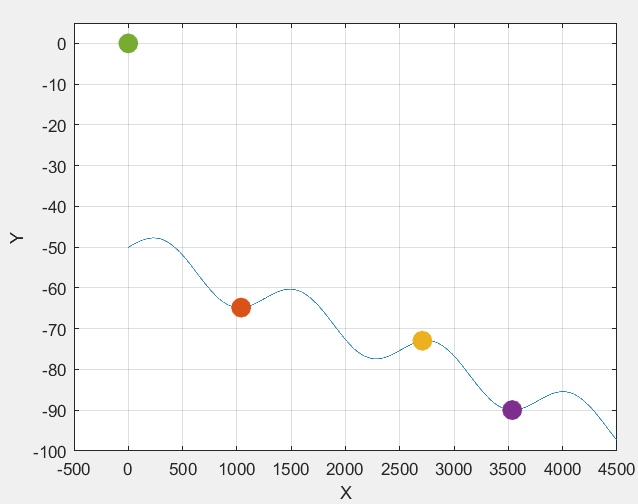
\includegraphics{Images/path.PNG}
	\caption{Map of the sea}
	\label{fig:map}
\end{figure}

Green dot is the start position of the submarine (0, 0). Every other colored dot on map is one habitat you have to visit. Blue line represents bottom of the sea so you have to be careful and not drive your submarine into it. We also provide you with the funtion used to generate the bottom : $0.01*(500*sin(0.005*X)-X) - 50$. Y level zero is the surface of the sea. 

Coliding with the sea bottom is instant fail.

\begin{table}[h!]
	\hyphenpenalty 10000
	\caption{Habitats and coordinates}
	\label{tab:nominalValues}
	\begin{tabularx}{\textwidth}{|Y|Y|Y|} \hline
		\textbf{Habitat} & X[m] & Y[m] \\ \hline 
		\textbf{Red} & 1039   & -64.82\\ \hline 
		\textbf{Yellow} & 2708  & -72.95\\ \hline
		\textbf{Purple} & 3535  &  -89.96\\ \hline
	\end{tabularx}
\end{table}



\begin{figure}[h!]
	\centering
	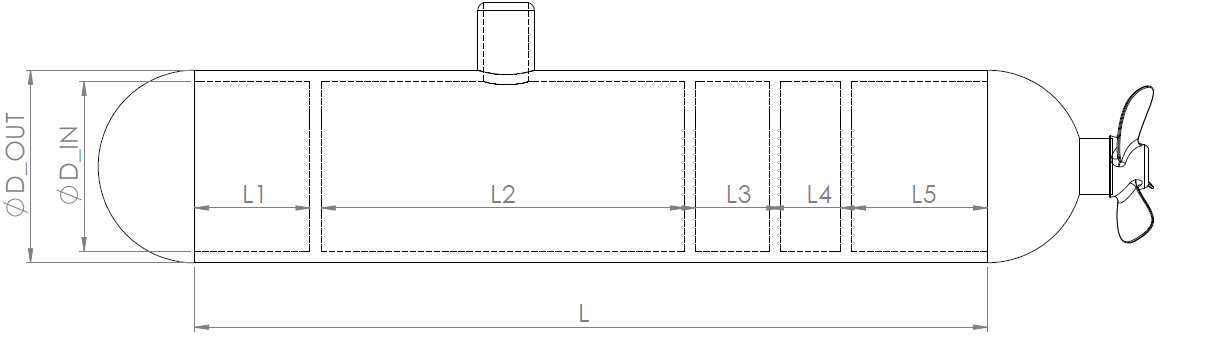
\includegraphics[width=\textwidth]{submarine_side_view.png}
	\caption{Submarine dimensions}
	\label{fig:side_view}
\end{figure}

The following dimensions are given:
\begin{itemize}
	\item $L = 15 \,\textrm{m}$
	\item $D_{OUT} = 3.4 \,\textrm{m}$
	\item $D_{IN} = 3 \,\textrm{m}$
	\item $m = 104.419$ t
	\item $balast\ volume = 30 \ m^3$
	\item $balast\ equilibrium = 50\%$
	\item $ballast\ fill\ speed = 100$ l/s
\end{itemize}


\textbf{Driving references are in this order} : $Red, Yellow, Purple$.


To help you in designing your driving function, GUI will be provided. GUI will allow you to change the submarine inputs and see how the submarine behaves.

Based on that, you have to design a regulator as a matlab function with prototype given in your task's folder.

Function output:

\begin{itemize}
	\item[Fuel percentage] - ${0.35,1}$ - Desired \% of fuel pump speed
	\item[Angle] - ${-7,7}$ - In degrees, vector of the output thrust
	\item[Target balast fill] - ${0,1}$ - Desired balast fill \%, the tank fills and empties with the $ballast\ fill\ speed$
	\item[Motor stop] - If this value is 0, the propulsion motor is shut down
	\item[Reverse] - If this value is negative, propulsion motor is reversed
\end{itemize}

Function input:

\begin{itemize}
	\item[pointIndex] - Index of habitat that is current reference point($[1, 2, 3]$ for [$Red, Yellow, Purple$], respectively)
	\item[vx, vy] - X and Y speeds
	\item[sx, sy] - X and Y positions
\end{itemize}


We will grade you \textbf{only by time} to perform whole trip.
	
	
	
\end{document}
